%\documentclass[a4paper,UKenglish,cleveref, autoref, thm-restate]{lipics-v2019}
\documentclass[manuscript,screen,review]{acmart}

%% \BibTeX command to typeset BibTeX logo in the docs
\AtBeginDocument{%
  \providecommand\BibTeX{{%
    \normalfont B\kern-0.5em{\scshape i\kern-0.25em b}\kern-0.8em\TeX}}}


%% Rights management information.  This information is sent to you
%% when you complete the rights form.  These commands have SAMPLE
%% values in them; it is your responsibility as an author to replace
%% the commands and values with those provided to you when you
%% complete the rights form.
\setcopyright{acmcopyright}
\copyrightyear{2018}
\acmYear{2018}
\acmDOI{10.1145/1122445.1122456}

%% These commands are for a PROCEEDINGS abstract or paper.
\acmConference[Woodstock '18]{Woodstock '18: ACM Symposium on Neural
  Gaze Detection}{June 03--05, 2018}{Woodstock, NY}
\acmBooktitle{Woodstock '18: ACM Symposium on Neural Gaze Detection,
  June 03--05, 2018, Woodstock, NY}
\acmPrice{15.00}
\acmISBN{978-1-4503-XXXX-X/18/06}


%\usepackage[utf8]{inputenc}
\usepackage{amsmath}
%\usepackage{amssymb}
\usepackage{amsthm}
\usepackage{graphicx}
%\usepackage[colorinlistoftodos]{todonotes}
\usepackage{algorithm}
\usepackage[noend]{algpseudocode}
%\usepackage{authblk}
%\usepackage{enumerate}
\usepackage{xcolor}
\usepackage{framed}
\usepackage{bm}
\usepackage{pifont}
\usepackage{multicol}
\usepackage{lipsum}
\usepackage{tikz}
\usetikzlibrary{calc}
\usepackage{wrapfig}
\usepackage{array}
%\usepackage[margin=1in]{geometry}
\usepackage{mathtools}
\usepackage{url}
\usepackage{thm-restate}
\usepackage{varwidth}
\usepackage{dsfont}

% \usepackage{subfig}

\usepackage{esvect}
\usepackage{enumitem}
\usepackage[strict]{changepage}

%\usepackage[pdftex]{hyperref}
%\usepackage[hidelinks]{hyperref}
\usepackage{caption}
\usepackage{subcaption}
\usepackage{anyfontsize}

\usepackage{afterpage}

% \newtheorem{observation}{Observation}
% \newtheorem{claim}{Claim}
\newtheorem{notation}{Notation}
\newtheorem{invariant}{Invariant}
% \newtheorem{definition}{Definition}
\newtheorem{assertion}{Assertion}
% \newtheorem{thm}{Theorem}
% \newtheorem{lemma}{Lemma}

\newcommand{\inred}[1]{{\color{red}{#1}}}
\newcommand{\inblue}[1]{{\color{blue}{#1}}}
\newcommand{\ingray}[1]{{\color{gray}{#1}}}
\newcommand{\remove}[1]{}
\newcommand\Set[2]{\{\,#1 \mid #2\,\}}
\newcommand\Collection[1]{\{\,#1\,\}}
\newcommand{\abs}[1]{\lvert#1\rvert}
\newcommand{\floor}[1]{{\left\lfloor {#1} \right\rfloor}}
\newcommand{\Int}{\int\limits}
\DeclareMathOperator*{\argmax}{arg\,max}

\declaretheorem[name=Theorem]{rthm}
% \declaretheorem[name=Claim]{clm}

\algblock{Vars}{EndFor}
\algrenewtext{Vars}{variables}
\algrenewtext{EndVars}{}
\algblock{ForEach}{EndFor}
\algrenewtext{ForEach}{for each }

% \newtheorem{observation}{Observation}
%\newtheorem{claim}{Claim}
%\newtheorem{definition}{Definition}
%\newtheorem{lemma}{Lemma}
\newtheorem{crly}{Corollary}


\declaretheorem[name=Claim]{clm}
\declaretheorem[name=Corollary]{crly2}


\newcommand{\CM}[4]{
    \begin{tikzpicture}[baseline=3ex]
        \draw[step=0.5cm,color=gray] (0,0) grid (1,1);
        \node at (0.25,0.25) {#3};
        \node at (0.25,0.75) {#1};
        \node at (0.75,0.75) {#2};
        \node at (0.75,0.25) {#4};
    \end{tikzpicture}
}

\newcommand{\orif}[1]{\textcolor{green}{[#1 -- ORI-FIXED]}}
\newcommand{\ori}[1]{\textcolor{red}{[#1 -- ORI]}}
\newcommand{\arik}[1]{\textcolor{red}{[#1 -- ARIK]}}
\newcommand{\dor}[1]{\textcolor{purple}{[#1 -- DOR]}}
\newcommand{\dorf}[1]{\textcolor{orange}{[#1 -- DOR-FIXED]}}

\newcommand{\forRevThree}[1]{{#1}}


\def \myScale {0.82}

\newcommand{\ingreen}[1]{{#1}}

\newcommand\diag[4]{%
  \multicolumn{1}{p{#2}|}{\hskip-\tabcolsep
  $\vcenter{\begin{tikzpicture}[baseline=0,anchor=south west,inner sep=#1]
  \path[use as bounding box] (0,0) rectangle (#2+2\tabcolsep,\baselineskip);
  \node[minimum width={#2+2\tabcolsep-\pgflinewidth},
        minimum  height=\baselineskip+\extrarowheight-\pgflinewidth] (box) {};
  \draw[line cap=round] (box.north west) -- (box.south east);
  \node[anchor=south west] at (box.south west) {#3};
  \node[anchor=north east] at (box.north east) {#4};
 \end{tikzpicture}}$\hskip-\tabcolsep}}



\newcommand{\fixed}[1]{\vskip 4mm \noindent{\color{blue} \textbf{Response:} {#1}} \vskip 5mm}
%\newcommand{\notfixed}[1]{\todo[inline,linecolor=red,backgroundcolor=red!5,bordercolor=red]{ {\footnotesize NOT FIXED: {#1}}}}

%\newcommand \fixed[1]{{\noindent\color{blue}#1}}

\newcommand \reviewer[1]{{\noindent\color{black}#1}}


%\renewcommand \ori[1]{}
%\renewcommand \janos[1]{}

\newcommand{\hash}{\mathpzc{h}}
%\newcommand{\deth}{\mathpzc{k}}
\newcommand{\deth}{\hat{h}}

\newcommand{\citetext}[1]{\protect\begin{mdframed}[leftmargin=1cm,rightmargin=1cm,shadow=true,shadowcolor=black!20,shadowsize=4pt] {\footnotesize \color{black} #1 } \protect\end{mdframed}}


\newcommand \prob{\mathbb{P}}
%%%%%%%%%%%%%%%%%%%%%%%%%%




\pgfplotsset{compat=1.16}

\begin{document}

%\nolinenumbers

\title{Intermediate Value Linearizability: A Quantitative Correctness Criterion}
\titlenote{An extended abstract describing this result
appears in DISC 2021 with the same authors and title.
The current version contains some missing proofs that are absent in the extended abstract,
the definition of IVL now uses posets as opposed to totally ordered sets.
Furthermore, we discuss other IVL objects (Sections~\ref{ivl-ssec:countMin}, \ref{ivl-ssec:sets-and-iterators}, and \ref{ivl-ssec:priority-q}).
}
%with Lightweight Synchronization}


%for Data Sketches and More}
%\titlerunning{Intermediate Value Linearizability} %TODO optional, please use if title is longer than one line

\author{Arik Rinberg}
\affiliation{%
  \institution{Technion}
  \streetaddress{}
  \city{Haifa}
  \country{Israel}}
\email{ArikRinerg@campus.technion.ac.il}

\author{Idit Keidar}
\affiliation{%
  \institution{Technion}
  \streetaddress{}
  \city{Haifa}
  \country{Israel}}
\email{idish@ee.technion.ac.il}

%\author{Arik Rinberg}{Technion, Israel}{ArikRinerg@campus.technion.ac.il}{}{}
%\author{Idit Keidar}{Technion, Israel}{idish@ee.technion.ac.il}{}{}

\renewcommand{\shortauthors}{A. Rinberg and I. Keidar}

\begin{abstract}
    
Big data processing systems often employ batched updates and data sketches to estimate certain properties of large data. For example, a \emph{CountMin sketch} approximates the frequencies at which elements occur in a data stream, and a \emph{batched counter} counts events in batches. This paper focuses on correctness criteria for concurrent implementations of such objects. Specifically, we consider \emph{quantitative} objects, whose return values are from an ordered domain, with a particular emphasis on \emph{$(\epsilon,\delta)$-bounded} objects that estimate a numerical quantity with an error of at most $\epsilon$ with probability at least $1 - \delta$.

The de facto correctness criterion for concurrent objects is linearizability. Intuitively, under linearizability, when a read overlaps an update, it must return the object's value either before the update or after it. Consider, for example, a single batched increment operation that counts three new events, bumping a batched counter's value from $7$ to $10$. In a linearizable implementation of the counter, a read overlapping this update must return either $7$ or $10$. We observe, however, that in typical use cases, any \emph{intermediate} value between $7$ and $10$ would also be acceptable. To capture this additional degree of freedom, we propose \emph{Intermediate Value Linearizability (IVL)}, a new correctness criterion that relaxes linearizability to allow returning intermediate values, for instance $8$ in the example above. Roughly speaking, IVL allows reads to return any value that is bounded between two return values that are legal under linearizability. 

A key feature of IVL is that we can prove that concurrent IVL implementations of
$(\epsilon,\delta)$-bounded objects are themselves $(\epsilon,\delta)$-bounded.
To illustrate the power of this result, we give a straightforward
and efficient concurrent implementation of an $(\epsilon, \delta)$-bounded
CountMin sketch, which is IVL (albeit not linearizable). 

We present four examples for IVL objects, each showcasing a different
way of using IVL. The first is a simple wait-free IVL batched counter, with $O(1)$ step complexity
for update. The next considers an $(\epsilon, \delta)$-bounded CountMin sketch, and further
shows how to relax IVL using \inred{the notion of} $r$-relaxation. Our third example is a non-atomic iterator
over a data structure. In this example, we augment the data structure with an \emph{auxiliary history variable}
state that includes ``tombstones'' for items deleted from the data structure. Here, IVL
semantics are required at the augmented level. Finally, using a \emph{priority queue},
we show that some objects require IVL to be paired with other correctness criteria;
indeed a natural correctness notion for a concurrent priority queue is IVL coupled
with sequential consistency.

Lastly, we show that IVL allows for inherently cheaper implementations
than linearizable ones. In particular, we show a lower bound of $\Omega(n)$
on the step complexity of the update operation of any wait-free linearizable
batched counter from single-writer multi-reader registers, which is more expensive than our $O(1)$ IVL implementation.
\end{abstract}



%\authorrunning{A. Rinberg and I. Keidar} %TODO mandatory. First: Use abbreviated first/middle names. Second (only in severe cases): Use first author plus 'et al.'

%\Copyright{Arik Rinberg and Idit Keidar} %TODO mandatory, please use full first names. LIPIcs license is "CC-BY";  http://creativecommons.org/licenses/by/3.0/

%\acknowledgements{We thank
%Hagit Attiya and Gadi Taubenfeld for their
%insightful comments, and the anonymous reviewers
%for their detailed feedback.}

\begin{CCSXML}
<ccs2012>
<concept>
<concept_id>10010147.10011777</concept_id>
<concept_desc>Computing methodologies~Concurrent computing methodologies</concept_desc>
<concept_significance>500</concept_significance>
</concept>
<concept>
<concept_id>10010520.10010521.10010528</concept_id>
<concept_desc>Computer systems organization~Parallel architectures</concept_desc>
<concept_significance>500</concept_significance>
</concept>
<concept>
<concept_id>10003752.10010124</concept_id>
<concept_desc>Theory of computation~Semantics and reasoning</concept_desc>
<concept_significance>500</concept_significance>
</concept>
<concept>
<concept_id>10003752.10003809.10011778</concept_id>
<concept_desc>Theory of computation~Concurrent algorithms</concept_desc>
<concept_significance>500</concept_significance>
</concept>
<concept>
<concept_id>10003752.10003809.10010055</concept_id>
<concept_desc>Theory of computation~Streaming, sublinear and near linear time algorithms</concept_desc>
<concept_significance>300</concept_significance>
</concept>
</ccs2012>
\end{CCSXML}
  
\ccsdesc[500]{Computing methodologies~Concurrent computing methodologies}
\ccsdesc[500]{Computer systems organization~Parallel architectures}
\ccsdesc[500]{Theory of computation~Semantics and reasoning}
\ccsdesc[500]{Theory of computation~Concurrent algorithms}
\ccsdesc[300]{Theory of computation~Streaming, sublinear and near linear time algorithms}

% \begin{CCSXML}
%     <ccs2012>
%      <concept>
%       <concept_id>10010520.10010553.10010562</concept_id>
%       <concept_desc>Computer systems organization~Embedded systems</concept_desc>
%       <concept_significance>500</concept_significance>
%      </concept>
%      <concept>
%       <concept_id>10010520.10010575.10010755</concept_id>
%       <concept_desc>Computer systems organization~Redundancy</concept_desc>
%       <concept_significance>300</concept_significance>
%      </concept>
%      <concept>
%       <concept_id>10010520.10010553.10010554</concept_id>
%       <concept_desc>Computer systems organization~Robotics</concept_desc>
%       <concept_significance>100</concept_significance>
%      </concept>
%      <concept>
%       <concept_id>10003033.10003083.10003095</concept_id>
%       <concept_desc>Networks~Network reliability</concept_desc>
%       <concept_significance>100</concept_significance>
%      </concept>
%     </ccs2012>
% \end{CCSXML}
    
% \ccsdesc[500]{Computer systems organization~Embedded systems}
% \ccsdesc[300]{Computer systems organization~Redundancy}
% \ccsdesc{Computer systems organization~Robotics}
% \ccsdesc[100]{Networks~Network reliability}

% \ccsdesc[500]{Theory of computation~Semantics and reasoning}
% \ccsdesc[500]{Computer systems organization~Parallel architectures}
% \ccsdesc[500]{Computing methodologies~Concurrent computing methodologies} %TODO mandatory: Please choose ACM 2012 classifications from https://dl.acm.org/ccs/ccs_flat.cfm



\keywords{concurrency, concurrent objects, linearizability} %TODO mandatory; please add comma-separated list of keywords

%\relatedversion{A full version of the paper is available at \cite{rinberg2020intermediate}, \url{https://arxiv.org/abs/2006.12889}.}



\maketitle




\chapter{Introduction}
\label{chap:intro}
% do we need to add TOC lines?

%\begin{figure}
%  \centering
%  \includegraphics[width=0.75\textwidth]{main/graphics/a_blowup.pdf}
%  \caption{This is a caption}
%\end{figure}

Here you can introduce the field, survey past results, give context, use citations of course... (e.g. \cite{Papadimitriou1994}). It is probably worthwhile to clarify the goals or targets of the research and describe the process, unless this is done later.

You can also introduce \emph{a key concept} (or rather, several) without formally defining them until later on.

\subsection*{An unnumbered subsection}

You may want to break up the intro into parts with titles. Subsectioning without numbering is an option you might want to consider.

Some people include a specific section overviewing the results ("In Chapter so-and-so, we will see how etc.") which is also a way of describing the structure of the thesis. But this is not necessary.

\subsection*{Thesis options and appearance}

Please note that the \texttt{iitthesis} class has several options when you use it, such as:
\begin{itemize}
\item \texttt{fullpageDraft} to avoid the margins necessary for proper binding when you make the final print
\item \texttt{beforeExam} makes the personal acknowledgements invisible; use this to print the copies you submit initially to the grad school for sending to the examiners (who shouldn't see these). For the final submission, drop this option.
\item \texttt{noabbrevs} no notation \& abbreviations list will be included in the thesis.
\end{itemize}


\section{Preliminaries}
\label{ivl-sec:preliminaries}

Section~\ref{ivl-ssec:det-objects} discusses deterministic shared memory objects and defines linearizability.
% the de facto standard correctness criterion,
%In Section~\ref{ivl-ssec:uni-step-complex} we define uniform step complexity, and in
In Section~\ref{ivl-ssec:rand-objects} we discuss randomized algorithms and their correctness criteria.

\subsection{Deterministic objects}
\label{ivl-ssec:det-objects}

We consider a standard shared memory model~\cite{herlihy1990linearizability}, where a set of \emph{asynchronous}
\emph{processes} access atomic shared memory variables. Accessing these
shared variables is instantaneous.
Processes take \emph{steps} according to an \emph{algorithm}, which is a deterministic
state machine, where a step can access a shared memory variable, do local computations, and possibly return
some value. \inred{A step may also alter the \emph{state}, which is it the collection of local and shared variables.}
 An \emph{execution} of an algorithm is an alternating
sequence of steps and states. We focus on algorithms that
implement \emph{objects}, which support
\emph{operations}, such as {\sc read} and {\sc write}. Operations begin
with an \emph{invocation} step and end with a \emph{response} step.
A \emph{schedule}, denoted $\sigma$, is the order in
which processes take steps, and the operations they invoke
in invoke steps with their parameters.
Because we consider deterministic algorithms,
$\sigma$ uniquely defines an execution of a given algorithm.

A \emph{history} is the sequence of invoke and response steps in an execution. Given an algorithm $A$ and
a schedule $\sigma$, $H(A, \sigma)$ is the history of the execution of $A$ with
schedule $\sigma$. A \emph{sequential} history is an alternating sequence of
invocations and their responses, beginning with an invoke step.
We denote the return value of operation $op$ with parameter $arg$ in history $H$ by $\text{ret}(x.op,H)$,
\inred{where $x$ is the object exposing operation $op$}.
We refer to the invocation step of operation $op$ with parameter $arg$
by process $p$ as $inv_p(x.op(arg))$ and to its response
step by $rsp_p(x.op(arg)\rightarrow ret)$, where $ret = \text{ret}(x.op,H)$, \inred{and where
$x$ in the object exposing operation $op$}. \inred{We omit $x$ and $arg$ when obvious from context.} A history
defines a partial order on operations: Operation $op_1$ \emph{precedes} $op_2$
in history $H$, denoted $op_1 \prec_H op_2$, if $rsp(op_1)$ precedes $inv(op_2(arg))$
in $H$. Two operations are \emph{concurrent} if neither precedes the other.

A \emph{well-formed} history is one that does not contain concurrent operations by the same process, and
where every response event for operation $op$ is preceded by an invocation of the same operation.
A schedule is well-formed if it gives rise to a well-formed history, and an execution
is well-formed if it is based on a well-formed schedule.
% The projection of a history $H$ onto an object $x$, denoted $H|_x$, is the
We denote by $H|_x$ the sub-history of $H$ consisting only of invocations and responses
on object $x$. Operation $op$ is \emph{pending} in a history $H$ if $op$ is invoked
in $H$ but does not return.

% A \emph{schedule}, generally denoted $\sigma$, is the order in
% which processes invoke operations or take steps. Given a deterministic algorithm, the schedule defines
% a history. A \emph{well-formed} schedule does not invoke concurrent operations by the same
% process, i.e., defines a well formed history.
% For some $op_i$, we define $\text{ret}(H, op_i)$ to be the return value of $op_i$
% in history $H$. The schedule is generated by the \emph{adversary}. For simplicity,
% we assume an \emph{oblivious} adversary, this adversary generates the schedule
% regardless of the observed coin flip vector.
% An object supports \emph{operations}, which are
% delimited by two events \emph{invoke} and \emph{response}.


% A \emph{register} supports the {\sc read} and {\sc write}($v$) operations.
% The response may return a value. A \emph{single writer multi reader (SWMR)} register has a predefined
% process which is the only one that is allowed to invoke a {\sc write} operation, but all processes may
% invoke a {\sc read} operation.


% %An invoke of operation $op$ by process $p$ is denoted $i_p^{op}$, similarly a response is denoted $r_p^{op}$.
% A \emph{history} $H$ is a sequence of invoke and response events. An example of a history with processes
% $p,q$ and a SWMR register which only process $p$ may write to can be $H=\mathit{inv}_p\text{\sc write}(3),
% \mathit{inv}_q\text{\sc read}, \mathit{rsp}_q\text{\sc read} \rightarrow 3, \mathit{rsp}_p\text{\sc write}$.
% For two operations $op_1,op_2$ in $H$, we say that $op_1$ \emph{precedes} $op_2$ in $H$, denoted
% $op_1 \prec_H op_2$, if the return even of $op_1$ precedes the invoke event of $op_2$ in $H$.
% Two operations are \emph{concurrent} if neither precedes the other.
% A \emph{well formed} history does not contain concurrent operations by the same process, and
% every response event for operation $op$ is preceded by an invocation of the same operation.
% The projection of a history $H$ onto and object $x$, denoted $H|_x$, is the sub-history consisting only of invocations and responses
% of operations on $x$.
% A \emph{sequential history} is a history in which each invocation is immediately followed
% by its response. The
% \emph{sequential specification} of an object is the set of its allowed sequential histories,
% denoted $\mathcal H$.

% Processes invoking operations take \emph{steps} according to an \emph{algorithm}, which is a deterministic
% state machine, where a step can access a shared variable, do local computations, and possibly return.
% A \emph{schedule}, generally denoted $\sigma$, is the order in
% which processes invoke operations or take steps. Given a deterministic algorithm, the schedule defines
% a history. A \emph{well formed} schedule does not invoke concurrent operations by the same
% process, i.e., defines a well formed history.
% For some $op_i$, we define $\text{ret}(H, op_i)$ to be the return value of $op_i$
% in history $H$. The schedule is generated by the \emph{adversary}. For simplicity,
% we assume an \emph{oblivious} adversary, this adversary generates the schedule
% regardless of the observed coin flip vector.

% Given a history $H$, an operation $op$ is said to be \emph{complete} if $H$ contains both
% $\mathit{inv}(op)$ and the corresponding $\mathit{rsp}(op)$. A history $H$ is said to
% be complete if all operations in it are complete, otherwise it is said to be incomplete.
% A well formed incomplete history $H$ can be completed to a history $H'$ by either removing
% incomplete operations or adding an appropriate response event, such that $\prec_H'$ 
% extends $\prec_H$. Given a history $H$, we denote the set of completed histories
% as $\mathit{complete}(H)$.


Correctness of an object's implementation is defined with respect to a
sequential specification $\mathcal{H}$, which is the object's set of allowed sequential histories.
If the history spans multiple objects, $\mathcal{H}$ consists of sequential histories $H$ such that for all
objects $x$, $H|_x$ pertains to $x$'s sequential specification (denoted $\mathcal{H}_x$).
A \emph{linearization}~\cite{herlihy1990linearizability} of a concurrent history $H$ is a
sequential history $H'$ such that (1) after removing some pending
operations from $H$ and completing others, it contains the same invocations and
responses as $H'$ with the same parameters and return values, and (2) $H'$
preserves the partial order $\prec_H$.
Note that our definition of linearization diverges from the one in~\cite{herlihy1990linearizability} in that
it is not associated with any sequential specification; instead we require that
the linearization pertain to the sequential specification when defining linearizability as follows:
Algorithm $A$ is a \emph{linearizable implementation}
of a sequential specification $\mathcal{H}$ if every history of a
well-formed execution of $A$ has a linearization in $\mathcal{H}$.

% If every concurrent well formed history has a linearization $H' \in {\mathcal H}$,
% then the object is said to be \emph{linearizable}. Furthermore, if any concurrent
% history $H$ arising from algorithm $A$ can be mapped to a sequential history $H'$ such
% that $H'$ is a sequential history arising from some atomic object $o$, then we say
% that algorithm $A$ \emph{implements} a linearizable object $o$.


% \subsection{Uniform step complexity}
% \label{ivl-ssec:uni-step-complex}

% We consider the strongest progress guarantee, \emph{bounded wait-freedom}.
% An operation is bounded wait-free if whenever a process
% invokes an operation, it completes (i.e., returns a response) in a bounded number of
% that process's steps, regardless of steps taken by other processes.
% An operation's \emph{step-complexity} is the maximum number of steps
% a process takes during a single execution of this operation. We
% can convert every bounded wait-free algorithm to a \emph{uniform step complexity}
% one, in which each operation takes the exact same
% number of steps in every execution. This can be achieved by padding shorter
% execution paths with empty steps before returning. For the remainder of this paper, we consider
% algorithms with uniform step complexity.

\subsection{Randomized algorithms}
\label{ivl-ssec:rand-objects}

% We next consider quantitative \emph{randomized} algorithms, where the return value of an
% operation is drawn from some distribution. Instead of a sequential
% specification, sequential randomized objects have error analyses, for example, the distance
% between the algorithms estimate of the number of distinct elements
% to the true value~\cite{KMV},
% or the distance between the lowest priority element and the true
% lowest priority~\cite{alistarh2015spraylist}.

In randomized algorithms, processes have access to coin flips from some domain $\Omega$.
Every execution is associated with a coin flip vector $\vv{c}=(c_1, c_2, \dots)$,
where $c_i \in \Omega$ is the $i^\text{th}$ coin flip in the execution.
A \emph{randomized algorithm} $A$ is a probability distribution over deterministic
algorithms $\{A({\vv{c})}\}_{{\vv{c}} \in \Omega^{\infty}}$\footnote{We do not consider non-deterministic objects in this paper.},
arising when $A$ is instantiated with different coin flip vectors.
% Similarly, a randomized sequential specification is a distribution over deterministic sequential specifications
% $\mathcal{H}(\vv{c})$ with coin flip vectors $\vv{c} \in \Omega^\infty$.
We denote by $H(A, {\vv{c}}, \sigma)$ the history of the execution of randomized algorithm
$A$ observing coin flip vector $\vv{c}$ in schedule $\sigma$.

% In randomized algorithms, one defines a notion of an \emph{adversary}, which
% selects the schedule (recall that the schedule includes invocations with their
% parameters, hence represents the algorithm's input).
% In this paper we focus on data sketches. These are randomized algorithms that almost
% invariably assume a \emph{weak adversary}, which selects the input
% independently of the random coin flips. We focus on weak adversaries in this paper.

% Under such an adversary,
% a randomized sequential algorithm A satisfies $\mathcal{H}$ if for
% every schedule $\sigma$, under a randomly sampled coin flip
% vector $\vv{c} \in \Omega^\infty$, $H(A,\vv{c},\sigma) \in \mathcal{H}(\vv{c})$. This
% means that for a given schedule $\sigma$, the distribution of return values
% in $A(\vv{c})$ is the same as in $\mathcal{H}(\vv{c})$. 


Golab et al. show that randomized algorithms that use concurrent objects require a stronger
correctness criterion than linearizability, and propose \emph{strong linearizability}~\cite{Wojciech}.
Roughly speaking, strong linearizability stipulates that the
mapping of histories to linearizations must be prefix-preserving,
so that future coin flips cannot impact the
linearization order of earlier events. In Definition~\ref{ivl-def:sivl}, we capture this notion
by requiring that the adversary decide on linearization points before observing the coin-flips.
% In this paper we focus on data sketches. These are randomized algorithms that almost
% invariably select the input independently of the random coin flips.
% Because weak adversaries cannot adapt to past coin flips,
% we can think of all coin flips as occurring ``in the future''.
% In this model, we can formulate strong linearizability
% to require that the linearization be independent of \emph{all} coin flips.
% We formalize this condition in Section~\ref{ivl-ssec:sivl}.


% \begin{definition}[Strong linearizability]
%     Let $H^?$ be a skeleton history of some randomized algorithm $A$ with schedule $\sigma$
%     (recall that the skeleton history is the same under all coin flip vectors).
%     $H^?$ is \emph{strongly linearizable} if there exists a linearization $H'$ such that for every coin flip
%     vector $\vv{c}$: $H'(\vv{c}) \in \mathcal{H}(\vv{c})$, and for every read $R$ that returns
%     in $H^?$: $\text{ret}(R, {H^?}(\vv{c})) = \text{ret}(R, {H'}(\vv{c}))$.

%     Algorithm $A$ is an \emph{strongly linearizable implementation} of a sequential specification distribution $\{\mathcal{H}\}_{\vv{c} \in \Omega^\infty}$ if every
%     history of a well-formed execution of $A$ is strongly linearizable with respect to $\{\mathcal{H}\}_{\vv{c} \in \Omega^\infty}$.
% \end{definition}

% An algorithm $A$ is a strongly linearizable implementation of object $o$ if
% for every history $H$ there exists a linearization $H' \in \mathcal{H}(\vv{c})_o$, and for every prefix
% $G$ of $H$ there exists a linearization $G' \in \mathcal{H}(\vv{c})_o$ of $G$ 
% such that $G'$ is a prefix of $H'$.

% In quantitative objects, randomization generally induces an \emph{error} on
% returned values. Further difficulty arises
% in analyzing the effect of parallelization on the error. Golab et al.
% show that linearization does not suffice for randomized objects~\cite{Wojciech}.
% They show that given the sequential error of a randomized object, the error guarantees
% do not hold for a linearizable one. Instead, they define
% define \emph{strong linearizability}~\cite{Wojciech}, a correctness
% criterion designed for randomized algorithms.
%Strong linearizability implies that
%the error analysis of the sequential object carries over to the concurrent one,
%as a strong adversary has the same strength for both a strongly linearizable implementation
%of an object and the same atomic one.


\section{Intermediate value linearizability}
\label{ivl-sec:ivl}

Section~\ref{ivl-ssec:definitions} introduces definitions that we utilize to define IVL.
Section~\ref{ivl-ssec:ivl} defines IVL for deterministic algorithms and proves that it is a local property.
Section~\ref{ivl-ssec:sivl} extends IVL for randomized algorithms, and Section~\ref{ivl-ssec:comparisons}
compares IVL to other correctness criteria.

\subsection{Definitions}
\label{ivl-ssec:definitions}

Our definitions use the notion of skeleton histories:
A \emph{skeleton history} is a sequence of invocation and response events, where the return values
of the responses are undefined, denoted $?$. For a history $H$, we define the operator $H^?$
as altering all response values in $H$ to $?$, resulting in a skeleton
history.
% Consider a randomized algorithm $A$, a schedule $\sigma$, and
% two coin flip vectors $\vv{c}, \vv{c}' \in \Omega^{\infty}$. From the uniform
% step complexity assumption, $\left[H(A, \vv{c}, \sigma)\right]^?=\left[H(A, \vv{c}', \sigma)\right]^?$,
% i.e., the skeleton history of a randomized algorithm's execution is uniquely determined by
% the schedule $\sigma$.

In this paper we discuss correctness criteria for a class of objects we call
\emph{quantitative}. These are objects that support two operations: (1) {\sc update},
which captures all mutating operations \inred{that do} not return a value; and (2) {\sc query},
which returns a value from some \emph{partially ordered set (poset)}. A poset
defines a partial relation between elements from the set, denoted $\leq$.
In Section~\ref{ivl-sec:examples} we exemplify our definitions for three types of return
values: (1) numerical values (a totally ordered domain), (2) sets of elements ordered
by containment (a partially ordered domain), and (3) ranked items stored in a priority
queue (a totally ordered domain).

In a \emph{deterministic quantitative object}
the return values of {\sc query} operations are uniquely defined. Namely, the object's sequential specification $\mathcal{H}$
contains exactly one history for every sequential history skeleton $H$; we denote this
history by $\tau_\mathcal{H}(H)$. Thus, $\tau_\mathcal{H}(H^?) = H$ for every history $H\in \mathcal{H}$.
Furthermore, for every sequential skeleton history $H$, by definition, $\tau_\mathcal{H}(H) \in \mathcal{H}$.
\inred{Note that if the object is not deterministic, $\tau_\mathcal{H}(H^?)$ isn't uniquely defined. We
use the following example to show how skeleton histories can be linearized and then converted back to histories:}

\begin{example}

Consider an execution in which a batched counter (formally defined in Section~\ref{ivl-ssec:lower-bound}) initialized to $0$
is incremented by $3$ by process $p$ concurrently with a query by
process $q$, which returns $0$. Its history is:
\[ H = inv_p(inc(3)), inv_q(query), rsp_p(inc), rsp_q(query \rightarrow 0). \]
The skeleton history $H^?$ is:
\[ H^? = inv_p(inc(3)), inv_q(query), rsp_p(inc), rsp_q(query \rightarrow ?). \]
A possible linearization of $H^?$ is:
\[ H'=inv_p(inc(3)), rsp_p(inc), inv_q(query), rsp_q(query \rightarrow ?). \]
Given the sequential specification $\mathcal{H}$ of a batched counter,
we get:
\[ \tau_\mathcal{H}(H')=inv_p(inc(3)), rsp_p(inc), inv_q(query), rsp_q(query \rightarrow 3). \]
In a different linearization, the query may return $0$ instead.

\end{example}

\subsection{Intermediate value linearizability}
\label{ivl-ssec:ivl}

% We consider objects supporting two operations, {\sc update} and {\sc query},
% where the former captures all mutating operations. Furthermore, all return
% values are from a totally ordered domain. We call such objects \emph{quantitative}
% objects. The return values in each sequential
% execution, i.e., the sequential specification $\mathcal{H}$, can be defined as a sequential
% deterministic algorithm $A$. By slight abuse of notation, we use $A$ as the
% sequential specification in this case. Given a deterministic algorithm
% $A$, this allows us to embody a sequential skeleton history $H^?$ by adding the
% correct return values, denoted $H^?(A)$, i.e., executing the operations on $A$ in the order
% that they happen in $H^?$. By definition, $H^?(A) \in \mathcal{H}$.

% We formalize correctness criteria for objects whose return values are from
% some \emph{partially ordered set (poset)}. A poset defines a partial relation between
% elements from the set, denoted $\leq$. An example of a poset is a power set over $S$,
% i.e., the set of all sets. In this case, the relation is $\subseteq$. A quantitative object is
% an example of such an object, as the \textsc{query}
% operation returns a value from a totally ordered domain.
We now define intermediate value linearizability.

% \begin{definition}[Intermediate value linearizability]
%   A history $H$ of an object is IVL with respect to sequential specification $\mathcal{H}$ if there
%   exist two linearizations $H_1, H_2$ of $H^?$ such that for every operation $o$ that returns a
%   value from some partially ordered set $(S, \leq)$ in $H$,
%   \[\text{ret}(o, \tau_\mathcal{H}(H_1)) \leq \text{ret}(o, H) \leq \text{ret}(o, \tau_\mathcal{H}(H_2)). \]

%   Algorithm $A$ is an \emph{IVL implementation} of a sequential specification $\mathcal{H}$ if every
%   history of a well-formed execution of $A$ is IVL with respect to $\mathcal{H}$.
%   \label{ivl-def:ivl}
% \end{definition}
    

\begin{definition}[Intermediate value linearizability]
  A history $H$ of an object is IVL with respect to sequential specification $\mathcal{H}$ if there
  exist two linearizations $H_1, H_2$ of $H^?$ such that for every {\sc query} $Q$
  that returns in $H$,
  \[\text{ret}(Q, \tau_\mathcal{H}(H_1)) \leq \text{ret}(Q, H) \leq \text{ret}(Q, \tau_\mathcal{H}(H_2)). \]

  Algorithm $A$ is an \emph{IVL implementation} of a sequential specification $\mathcal{H}$ if every
  history of a well-formed execution of $A$ is IVL with respect to $\mathcal{H}$.
  \label{ivl-def:ivl}
\end{definition}

Note that a linearizable object is trivially IVL, as the skeleton history of the linearization of $H$ plays the roles
of both $H_1$ and $H_2$. We emphasize that in a sequential execution, an IVL object is not relaxed
in any way -- it must follow the sequential specification. Similarly, in a well-formed history,
operations of the same process never overlap, and so IVL executions satisfy program order.

\inred{We now show that IVL is both local and non-blocking(as defined in~\cite{herlihy1990linearizability}):}
%The following theorem shows that this property is local (as defined in~\cite{herlihy1990linearizability}):
\begin{restatable}{thm}{local}
  \label{ivl-thm:ivl-local}
  A history $H$ of a well-formed execution of algorithm $A$ over a set of objects $\mathcal{X}$
  is IVL if and only if for each object $x \in \mathcal{X}$, $H|_x$ is IVL.
\end{restatable}
\begin{proof}
  Let $A$ be a deterministic algorithm, and let $\mathcal{H}_x$ be the sequential specification of object $x$, for every $x \in \mathcal{X}$.
  The ``only if'' part is immediate.

  Denote by ${H_1^x}, {H_2^x}$ the linearizations of ${H|_x}^?$ given by the
  definition of IVL.
  We first construct a linearization $H_1$ of $H^?$, \inred{i.e., the order $\prec_{H_1}$},
  as follows: For every pending operation on object $x$, we either
  add the corresponding response or remove it based on ${H_1^x}$. We then construct a partial order
  of operations as the union of $\{{\prec}_{H_1^x}\}_{x \in \mathcal{X}}$ and the realtime order
  of operations in $H$. As each ${\prec}_{H_1^x}$ must adhere to the realtime order of $H|_x$,
  and therefore $H$, and the set of operations $\{{\prec}_{H_1^x}\}_{x \in \mathcal{X}}$ are disjoint, this partial order
  is well defined. Consider two concurrent operations $op_1, op_2$ in $H$. If they
  do not belong to the same history $H|_x$ for some object $x$, we order them arbitrarily in $\prec_{H_1}$.
  We construct linearization $H_2$ of $H^2$ by defining the order of operations $\prec_{H_2}$ in a similar fashion,
  \inred{ where the added responses or removed pending operations are based on ${H_2^x}$ instead of ${H_1^x}$}.

  By construction all invocations and responses appearing in $H^?$ appear both in $H_1$ and in $H_2$,
  and $H_1$ and $H_2$ preserve the partial order $\prec_{H^?}$. Therefore, $H_1$ and $H_2$ are linearizations
  of $H^?$.
  
  Consider some read $R$ on some object $x \in \mathcal{X}$ that returns in $H$. As $H|_x$ is IVL
  $\text{ret}(R,  \tau_{\mathcal{H}_x}(H_1^x)) \leq \text{ret}(R, H|_x) \leq \text{ret}(R, \tau_{\mathcal{H}_x}(H_2^x))$.
  Note that $\text{ret}(R, H|_x) = \text{ret}(R, H)$.
  Furthermore, $\text{ret}(R, \tau_{\mathcal{H}_x}(H_1^x))= \text{ret}(R, \tau_{\mathcal{H}}(H_1))$
  and $\text{ret}(R, \tau_{\mathcal{H}_x}(H_2^x))= \text{ret}(R, \tau_{\mathcal{H}}(H_2))$,
  as objects other than $x$ do not affect the return value of this operation. Therefore $H$ is IVL.
\end{proof}
% \begin{theorem}
%   A history $H$ of a well-formed execution of algorithm $A$ over a set of objects $\mathcal{X}$
%   is IVL if and only if for each object $x \in \mathcal{X}$, $H|_x$ is IVL.
% \end{theorem}
% \begin{proof}
%   Let $A$ be a deterministic algorithm, and let $\mathcal{H}_x$ be the sequential specification of object $x$, for every $x \in \mathcal{X}$.
%   The ``only if'' part is immediate.

%   Denote by ${H_1^x}, {H_2^x}$ the linearizations of ${H|_x}^?$ guaranteed by the
%   definition of IVL.
%   We first construct a linearization $H_1$ of $H^?$, defined
%   by the order $\prec_{H_1}$ as follows: For every pending operation on object $x$, we either
%   add the corresponding response or remove it based on ${H_1^x}$. We then construct a partial order
%   of operations as the union of $\{{\prec}_{H_1^x}\}_{x \in \mathcal{X}}$ and the realtime order
%   of operations in $H$. As ${\prec}_{H_1^x}$ must adhere to the realtime order of $H|_x$,
%   and therefore $H$, and the order of operations in $\{{\prec}_{H_1^x}\}_{x \in \mathcal{X}}$ are disjoint, this partial order
%   is well defined. Consider two concurrent operations $op_1, op_2$ in $H$. If they
%   do not belong to the same history $H|_x$ for some object $x$, we order them arbitrarily in $\prec_{H_1}$.
%   We construct linearization $H_2$ of $H^2$ by defining the order of operations $\prec_2$ in a similar fashion.

%   By construction all invocations and responses appearing in $H^?$ appear both in $H_1$ and in $H_2$,
%   and $H_1$ and $H_2$ preserve the partial order $\prec_{H^?}$. Therefore, $H_1$ and $H_2$ are linearizations
%   of $H^?$.
  
%   Consider some read $R$ on some object $x \in \mathcal{X}$ that returns in $H$. As $H|_x$ is IVL
%   $\text{ret}(R,  \tau_{\mathcal{H}_x}(H_1^x) \leq \text{ret}(R, H|_x) \leq \text{ret}(R, \tau_{\mathcal{H}_x}(H_2^x))$.
%   Note that $\text{ret}(R, H|_x) = \text{ret}(R, H)$. Furthermore, $\text{ret}(R, \tau_{\mathcal{H}_x}(H_i^x))= \text{ret}(R, \tau_{\mathcal{H}}(H_i))$ for $i \in \{1,2\}$,
%   as objects other than $x$ do not affect the return value of this operation. Therefore $H$ is IVL.
% \end{proof}

Locality allows system designers to reason about their system in a modular fashion. Each object can be built separately,
and the system as a whole still satisfies the property.
\inred{
\begin{theorem}
  \label{ivl-thm:ivl-non-blocking}
  Let $H$ be an IVL history of a well-formed execution of a algorithm $A$. If $inv_p(op(arg))$ is an invocation
  of a pending operation in $H$, then there exists $rsp_p(op)\rightarrow ret$ such that $H \cdot rsp_p(op)\rightarrow ret$
  is IVL.
\end{theorem}
\begin{proof}
  Let $H$ be an IVL history of a well-formed execution of a algorithm $A$. Let $inv_p(op(arg))$ be an invocation
  of a pending operation in $H$. If the invocation is not that of a {\sc query} operation, then
  $H \cdot rsp_p(op)\rightarrow \bot$ is IVL. Otherwise,  denote the query as $Q$.
  
  Let $H^?$ be the skeleton history of $H$. Denote $H' = H^? \cdot rsp_p(op)\rightarrow ?$.
  Note that $H'$ is also a skeleton history. Let $H''$ be some linearization of $H'$. Finally, let
  $v=\text{ret}(Q, \tau_\mathcal{H}(H''))$. Then, $H \cdot rsp_p(op)\rightarrow v$ is IVL,
  where $H_1=H_2=H''$.
\end{proof}
}

\subsection{Extending IVL for randomized algorithms}
\label{ivl-ssec:sivl}

% the specification of the deterministic algorithm $A(\vv{c})$ is given
% by the deterministic sequential specification $\mathcal{H}(\vv{c})$.
% Thus, a randomized sequential specification is a distribution over deterministic sequential specifications
% $\mathcal{H}(\vv{c})$ with coin flip vectors $\vv{c} \in \Omega^\infty$, i.e., a distribution over

% A randomized sequential specification is a distribution over deterministic sequential specifications
% $\mathcal{H}(\vv{c})$ with coin flip vectors $\vv{c} \in \Omega^\infty$. Recall that we consider
% a weak adversary in this paper. Under such an adversary,
% a randomized sequential algorithm A satisfies $\mathcal{H}$ if for
% every schedule $\sigma$, under a randomly sampled coin flip
% vector $\vv{c} \in \Omega^\infty$, $H(A,\vv{c},\sigma) \in \mathcal{H}(\vv{c})$. This
% means that for a given schedule $\sigma$, the distribution of return values
% in $A(\vv{c})$ is the same as in $\mathcal{H}(\vv{c})$.

\inred{For the remainder of this paper we consider the strongest progress guarantee, bounded wait-freedom.
\inred{An operation $op$ is \emph{wait-free} if whenever a process $p$ invokes $op$, $op$ returns
a response regardless of steps taken by other processes.}
An operation $op$ is \emph{bounded wait-free} if whenever any process $p$
invokes $op$, $op$ returns a response in a bounded number of
$p$'s steps, regardless of steps taken by other processes.
An operation's \emph{step-complexity} is the maximum number of steps
a process takes during a single execution of this operation. We
can convert every bounded wait-free algorithm to a \emph{uniform step complexity}
one, in which each operation takes the exact same
number of steps in every execution.
This can be achieved by padding shorter
execution paths with empty steps before returning.
Note that in a randomized algorithm with uniform step complexity, coin flips have
no impact on $op$'s execution times.}

In a randomized algorithm $A$ with uniform step complexity, every invocation
of a given operation returns after the same number of steps,
regardless of the coin flip vector $\vv{c}$. This, in turn, implies that
for a given $\sigma$, for any $\vv{c}, \vv{c}' \in \Omega^{\infty}$, the
arising histories $H(A, \vv{c}, \sigma)$ and $H(A, \vv{c}', \sigma)$ differ only in the operations'
return values but not in the order of invocations and responses, as the latter is
determined by $\sigma$, so their skeletons are equal. For randomized algorithm $A$ and schedule $\sigma$,
we denote this arising skeleton history by $H^?(A, \sigma)$.
% Furthermore, for any two coin flip vectors $\vv{c}, \vv{c}' \in \Omega^{\infty}$,
% $H^?(A, \sigma) \triangleq \left[H(A, \vv{c}, \sigma)\right]^?=\left[H(A, \vv{c}', \sigma)\right]^?$.

We are faced with a dilemma when defining the specification
of a randomized algorithm $A$, as the algorithm itself is a distribution over a
set of algorithms $\{A(\vv{c})\}_{\vv{c}\in \Omega^\infty}$. Without knowing
the observed coin flip vector $\vv{c}$, the execution behaves unpredictably. We therefore
define a deterministic sequential specification $\mathcal{H}(\vv{c})$ for each coin flip vector
$\vv{c} \in \Omega^\infty$, so the sequential specification is a
probability distribution on a set of sequential histories $\{\mathcal{H}(\vv{c})\}_{\vv{c}\in \Omega^\infty}$.

% For randomized algorithm $A$, a schedule $\sigma$, we denote this skeleton history
% by $H^?(A, \sigma)$, i.e., $[H(A, \sigma, \vv{c})]^?=H^?(A , \sigma)$
% for any $\vv{c} \in \Omega^\infty$.

% and a coin flip vector $\vv{c} \in \Omega^\infty$

% Therefore, for a randomized algorithm $A$, a schedule $\sigma$, and
% two coin flip vectors $\vv{c}, \vv{c}' \in \Omega^{\infty}$, 
% $H^?(A, \sigma) \triangleq \left[H(A, \vv{c}, \sigma)\right]^?=\left[H(A, \vv{c}', \sigma)\right]^?$.
% We denote this skeleton history by $H^?(A, \sigma)$.

% In contrast to deterministic objects, where we defined a linearization for each history,
% randomized algorithms require a common linearization for each skeleton history
% that will hold true under all possible coin flip vectors.
% We define
% strong linearizability using the linearization of the skeleton history:
% \begin{definition}[Strong linearizability]
%   Consider a skeleton history $H=H^?(A, \sigma)$ of some
%   randomized algorithm $A$ with schedule $\sigma$.
%   $H$ is \emph{strongly linearizable} with respect to $\{\mathcal{H}(\vv{c})\}_{\vv{c} \in \Omega^\infty}$ if there exists a
%   linearization $H'$ of $H$ such that for every coin flip vector $\vv{c}$ and read $R$
%   that returns in $H$: $\text{ret}(R, \tau_{\mathcal{H}(\vv{c})}(H')) = \text{ret}(R, H(A, \vv{c}, \sigma))$.

%   Algorithm $A$ is a \emph{strongly linearizable implementation} of a sequential specification distribution $\{\mathcal{H}(\vv{c})\}_{\vv{c} \in \Omega^\infty}$ if every
%   skeleton history of a well-formed execution of $A$ is strongly linearizable with respect to $\{\mathcal{H}(\vv{c})\}_{\vv{c} \in \Omega^\infty}$.
% \end{definition}
% As linearizable objects are, in particular, IVL, we must strengthen IVL in a similar manner. We call this
% stronger variant \emph{strong intermediate value linearizability (SIVL)}:

A correctness criterion for randomized objects needs to capture the property that the distribution of
a randomized algorithm's outcomes matches the distribution of behaviors allowed by the specification.
Consider, e.g., some sequential skeleton history $H$ of an object defined by $\{\mathcal{H}(\vv{c})\}_{\vv{c}\in \Omega^\infty}$. Let Q be a query
that returns in $H$, and assume that $Q$ has some probability $p$ to return a value $v$ in $\tau_{\mathcal{H}(\vv{c})}(H)$ for
a randomly sampled $\vv{c}$. Intuitively, we would expect that if a randomized algorithm $A$ ``implements'' the specification
$\{\mathcal{H}(\vv{c})\}_{\vv{c}\in \Omega^\infty}$, then $Q$ has a similar probability to return $v$ in sequential executions of $A$ with the same history,
and to some extent also in concurrent executions of $A$ of which $H$ is a linearization. In other words, we
would like the distribution of outcomes of $A$ to match the distribution of outcomes in $\{\mathcal{H}(\vv{c})\}_{\vv{c}\in \Omega^\infty}$.
\inred{For example, consider a sequential specification that allows returns $0$ with probability $0.5$, and $1$ with probability $0.5$. For an
algorithm to implement such an object, it is not enough for it to return only $0$ or $1$, but we expect $0$ to be returned with
probability $0.5$, and $1$ to be returned with probability $0.5$.}


We observe that in order to achieve this, it does not suffice to require that each history has an
arbitrary linearization as we did for deterministic objects, because this might not preserve the
desired distribution \inred{as is shown in~\cite{Wojciech}}. Instead, for randomized objects we require a common linearization for each
skeleton history that will hold true under all possible coin flip vectors.
\inred{In other words, the linearization is independent of the coin flip vector.}
We therefore formally
define IVL for randomized objects as follows:

% \begin{definition}[IVL for randomized algorithms]

%   Consider a skeleton history $H=H^?(A, \sigma)$ of some
%   randomized algorithm $A$ with schedule $\sigma$.
%   $H$ is \emph{IVL} with respect to $\{\mathcal{H}(\vv{c})\}_{\vv{c} \in \Omega^\infty}$ if there exist
%   linearizations $H_1, H_2$ of $H$ such that for every coin flip vector $\vv{c}$ and some operation $o$
%   that returns a value from some partially ordered set $(S, \leq)$ in $H$,
%   \[\text{ret}(o, \tau_{\mathcal{H}(\vv{c})}(H_1)) \leq \text{ret}(o, H(A, \vv{c}, \sigma)) \leq \text{ret}(o, \tau_{\mathcal{H}(\vv{c})}(H_2)). \]

%   Algorithm $A$ is an \emph{IVL implementation} of a sequential specification
%   distribution $\{\mathcal{H}(\vv{c})\}_{\vv{c} \in \Omega^\infty}$ if every skeleton
%   history of a well-formed execution of $A$ is IVL with
%   respect to $\{\mathcal{H}(\vv{c})\}_{\vv{c} \in \Omega^\infty}$.
%   \label{ivl-def:sivl}
% \end{definition}

\begin{definition}[IVL for randomized algorithms]
  Consider a skeleton history $H=H^?(A, \sigma)$ of some
  randomized algorithm $A$ with schedule $\sigma$.
  $H$ is \emph{IVL} with respect to $\{\mathcal{H}(\vv{c})\}_{\vv{c} \in \Omega^\infty}$ if there exist
  linearizations $H_1, H_2$ of $H$ such that for every coin flip vector $\vv{c}$ and query $Q$
  that returns in $H$,
  \[\text{ret}(Q, \tau_{\mathcal{H}(\vv{c})}(H_1)) \leq \text{ret}(Q, H(A, \vv{c}, \sigma)) \leq \text{ret}(Q, \tau_{\mathcal{H}(\vv{c})}(H_2)). \]

  Algorithm $A$ is an \emph{IVL implementation} of a sequential specification
  distribution $\{\mathcal{H}(\vv{c})\}_{\vv{c} \in \Omega^\infty}$ if every skeleton
  history of a well-formed execution of $A$ is IVL with
  respect to $\{\mathcal{H}(\vv{c})\}_{\vv{c} \in \Omega^\infty}$.
  \label{ivl-def:sivl}
\end{definition}

% Note that the query $Q$ in Definition~\ref{ivl-def:sivl} is not necessarily ``correct''; rather,
% it is bounded between two (possibly erroneous) results returned in linearizations.
\inred{Since we require a common linearization of the skeleton histories under all coin flips vectors,
the linearizations are a foriori independent of future coin flips. Hence, an adversary cannot affect
the linearization based on observing the coin flip vector.}

% Since we require a common linearization under all coin flip vectors, we do not need to
% strengthen IVL for randomized settings in the manner that strong linearizability
% strengthens linearizability. This is because the linearizations we consider are a fortiori independent of future coin flips.
% \inred{In other words, the range of admissible behaviors is determined by variation in the interleaving steps, and not
% by the variation  in coin flips. Definition~\ref{ivl-def:sivl} is both local and non-blocking, with a similar proof to Definition~\ref{ivl-def:ivl}.}

% Note that a strongly linearizable object is trivially SIVL, as the linearization of $H$ plays the role of both $H_1$ and $H_2$.

% We show that for a certain family of objects, the error of a sequential
% object remains bounded in a concurrent SIVL implementation.
% We first define the family, which we denote \emph{$\delta$-bounded} randomized
% objects, as follows. Let $o$ be a sequential randomized object, and let $H^?$ be
% some arising skeleton history from schedule $\sigma$.
% Consider any read $R$ that completes in $H^?$. We say that $R$ is bounded if
% there exist $v_1, v_2$ such that with probability
% $\geq 1-\delta$, $R$ returns $v$ in $H^?_{\vv{c}}$ such that $v_1 \leq v \leq v_2$,
% for some sampled $\vv{c} \in \Omega^{\infty}$. If this is true for every completed read $R$ in $H^?$,
% then we say that $H^?$ is $\delta$-bounded. If every history arising for an
% execution of $o$ is $\delta$-bounded, then we say that
% $o$ is a \emph{$\delta$-bounded} randomized object.

% We now show the following theorem:
% \begin{theorem}
%   Let $o$ be a sequential object, and let algorithm $A$ be an SIVL implementation
%   of $o$. If $o$ is a $\delta$-bounded randomized object, then $A$ is a $2\delta$-bounded
%   randomized object.
%   \label{ivl-thm:SIVL-bound}
% \end{theorem}
% \begin{proof}
%   Let $o$ be a $\delta$-bounded randomized sequential object, and let $A$ be an SIVL implementation
%   of $o$. Let $\vv{c}$ be a coin flip vector, and let $\sigma$ be a schedule. Consider $H(\vv{c}, \sigma)$,
%   the concurrent history arising from an execution of $A$. Consider some operation $R$ that returns some value in $H(\vv{c}, \sigma)$.

%   Consider the skeleton history $H^?$ of $H(\vv{c}, \sigma)$. As $A$ is SIVL there exist linearizations
%   $H_1^?, H_2^?$ of $H^?$, such that
%   $\text{ret}(R, {H_1^?}(\vv{c})) \leq \text{ret}(R, {H^?}(\vv{c})) \leq \text{ret}(R, {H_2^?}(\vv{c}))$.
%   Note that $H_i^?(\vv{c})$ is a sequential history of $A$. As such, we can execute the operations on object
%   $o$ in the same order and observing the some coin flip vector $\vv{c}$ and arrive at history $H'$
%   such that $H'=H_i^?(\vv{c})$ for $i \in \{1,2\}$. As $o$ is a $\delta$-bounded randomized object, there exit values
%   $v_i^1, v_i^2$ such that $v_i^1 \leq \text{ret}(H_i^?(\vv{c})) \leq v_i^2$ with probability $\geq 1-\delta$, for $i \in \{1,2\}$.
%   Therefore, $v^1 \leq v_1^1$ and with probability $\leq \delta$: $v^2 \geq v_2^2$.
%   As $A$ is an SIVL implementation of $o$, there exist linearizations $H_1,H_2$,
%   and values $v^1,v^2$ such that $v^1 \leq v \leq v^2$. As $H_1$ and $H_2$ are sequential
%   histories, then there exists $v_1^1,v_2^1,v_1^2,v_2^2$ such that with probability
%   $\geq 1 - \delta$: $v_1^1 \leq v^1 \leq v_2^1$ and with probability
%   $\geq 1 - \delta$: $v_1^2 \leq v^2 \leq v_2^2$. Therefore, with probability $\leq \delta$:
%   $\text{ret}(H_1^?(\vv{c})) \leq v_1^1$ and with probability $\leq \delta$: $\text{ret}(H_2^?(\vv{c})) \geq v_2^2$.

%   Therefore,
%   with probability $\geq 1 - 2 \delta$ then both $\text{ret}(H_1^?(\vv{c})) \geq v_1^1$ and $\text{ret}(H_2^?(\vv{c})) \leq v_2^2$,
%   and therefore with probability $\geq 1 - 2 \delta$ then
%   $v_1^1 \leq \text{ret}(H_1^?(\vv{c})) \leq \text{ret}(H^?(\vv{c})) \leq \text{ret}(H_2^?(\vv{c})) \leq v_2^2$.
%   Meaning, choosing $v_1 = v_1^1$ and $v_2 = v_2^2$ proves the theorem.
% \end{proof}



% The importance we see in defining correctness criteria for randomized objects
% is twofold: the first is the ease of concurrent error relaxation and the
% second is the implementation flexibility it provides.
% \inred{ARIK: I'm trying to work out how to say that the error analysis of
% a strongly linearizable object is the same as an atomic one. I'm not sure how to
% say this.}

% Here too the sequential
% analysis carries over to the concurrent
% setting, with an additional relaxation error, i.e., the error that is added
% due to overtaking a bounded number of operations. Like strong linearizability, the analysis
% is relative to a sequential specification which is only applicable to a deterministic
% execution. While the flexibility is larger than that of strong linearizability,
% it is still bounded by a factor of $r$.

%  This framework does not
% leverage existing literature of the error in the sequential setting, which we
% wish to leverage.

\subsection{\texorpdfstring{$r$}{r}-relaxed IVL}
\label{ivl-ssec:relaxed-cm}

Henzinger et al. define $r$-relaxed semantics~\cite{Henzinger}.
Intuitively, each operation on the relaxed object is assigned a \emph{cost}. An
$r$-relaxation allows operations whose costs do not exceed $r$. Rinberg et al.~\cite{rinberg2019fast}
define the cost of some operation $o$ to be the number of operations that precede it in the
concurrent history, but do not precede it in the sequential one.
\inred{Paraphrasing} the definition of the $r$-relaxed
specification for some sequential specification $\mathcal{H}$ from Rinberg et al.~\cite{rinberg2019fast}:
\begin{definition}[r-relaxation]
    A sequential history $H$ is an \emph{$r$-relaxation} of a sequential history $H'$
    if $H$ is comprised of all the invocations in $H'$ and their responses,
    and each invocation in $H$ is preceded by all but at most $r$ of the invocations that precede the 
    same invocation in $H'$. The \emph{$r$-relaxation} of $\mathcal{H}$ is the set of histories
    that have r-relaxations in $\mathcal{H}$:
    
    $\mathcal{H}^r \triangleq $ $\{H'|\exists H\in$$\mathcal{H}$ s.t. $H$ is an $r$-relaxation of $H'\}$.
    \label{ivl-def:r-relaxtion}
\end{definition}
We can plug Definition~\ref{ivl-def:r-relaxtion} into Definition~\ref{ivl-def:sivl} instead
of the sequential specification there to get a specification for $r$-relaxed IVL objects.
For completeness, we define $r$-relaxed IVL:
\begin{definition}[$r$-Relaxed IVL]
  Consider a skeleton history $H=H^?(A, \sigma)$ of some
  randomized algorithm $A$ with schedule $\sigma$.
  $H$ is $r$-relaxed \emph{IVL} with respect to $\{\mathcal{H}^r(\vv{c})\}_{\vv{c} \in \Omega^\infty}$ if there exist
  linearizations $H_1, H_2$ of $H$ such that for every coin flip vector $\vv{c}$ and query $Q$
  that returns in $H$,
  \[\text{ret}(Q, \tau_{\mathcal{H}^r(\vv{c})}(H_1)) \leq \text{ret}(Q, H(A, \vv{c}, \sigma)) \leq \text{ret}(Q, \tau_{\mathcal{H}^r(\vv{c})}(H_2)). \]

  Algorithm $A$ is an $r$-relaxed \emph{IVL implementation} of a sequential specification
  distribution $\{\mathcal{H}(\vv{c})\}_{\vv{c} \in \Omega^\infty}$ if every skeleton
  history of a well-formed execution of $A$ is IVL with
  respect to $\{\mathcal{H}^r(\vv{c})\}_{\vv{c} \in \Omega^\infty}$.
  \label{ivl-def:relaxed-sivl}
\end{definition}
\inred{As Definition~\ref{ivl-def:relaxed-sivl} is IVL with respect to an r-relaxed specification, it is
both local and non-blocking.} In Section~\ref{ivl-ssec:countMin}, we show that this allows us to create more NUMA-friendly objects.



\subsection{Relationship to other relaxations}
\label{ivl-ssec:comparisons}

In spirit, IVL resembles the \emph{regularity} correctness condition for
single-writer registers~\cite{lamport1986interprocess}, where a query must return
either a value written by a concurrent write or the last value written
by a write that completed before the query began. Stylianopoulos  
et al.~\cite{stylianopoulos2020delegation} adopt a similar condition for data sketches, which they
informally describe as follows: ``a query takes into account all completed
insert operations and possibly a subset of the overlapping ones.''
If the object's estimated quantity (return value) is monotonically increasing
throughout every execution, then IVL essentially captures this condition,
while also allowing intermediate steps of a single update to be observed.
But this is not the case in general. Consider, for example, an
object supporting increment and decrement, and a query that occurs concurrently
with an increment and an ensuing decrement. If the query takes only the decrement
into account (and not the increment), it returns a value that is smaller than all legal return values
that may be returned in linearizations, which violates IVL. Our interval-based
formalization is instrumental to ensuring that a concurrent IVL implementation
preserves the probabilistic error bounds of the respective sequential sketch, which we prove in the next section.

Another example of an object specified in the spirit of IVL is Lamport's monotonic
clock~\cite{lamport1990concurrent}, where a read is required to return a value bounded between the clock's
values at the beginning and end of the read’s interval.

Previous work on set-linearizability~\cite{neiger1994set} and
interval-linearizability~\cite{castaneda2018unifying} has also relaxed linearizability,
allowing a larger set of return values in the presence of overlapping operations. The set of possible return
values, however, must be specified in advance by a given state machine; operations' effects
on one another must be predefined.
In fact, interval-linearizability could be used to define IVL on a per-object basis, by defining
a nondeterministic interval-sequential object in which a read operation can return any value in
the interval defined by the update operations that are concurrent with it. In
contrast, \inred{when considering quantitative objects,} IVL is generic and does not require
additional object-specific definitions; it provides an intuitive quantitative bound
on possible return values.

Henzinger et al.~\cite{Henzinger} define
the quantitative relaxation framework, which
allows executions to differ from the sequential specification up to a bounded cost function.
We use this framework when defining relaxed IVL.
Alistarh et al.
expand upon this and define \emph{distributional linearizability}~\cite{alistarh2018distributionally},
which requires a distribution over the internal
states of the object for its error analysis.
Rinberg et al. consider strongly linearizable $r$-relaxed semantics for randomized objects~\cite{rinberg2019fast}.
IVL differs from these definitions in two points: First, a sequential history of an IVL object
must adhere to the sequential specification, whereas in these
relaxations even a sequential history may diverge from the specification. The second is that these relaxations
are measured with respect to a single linearization. We, instead, bound
the return value between two legal linearizations. The latter is the key to preserving the
error bounds of sequential objects, as we next show.

\section{\texorpdfstring{$(\epsilon,\delta)$}{(epsilon,delta)}-bounded objects}
\label{ivl-sec:bounded-objects}

In this section we show that for a large class of randomized objects,
IVL concurrent implementations preserve the error bounds of the respective
sequential ones. More specifically, we focus on randomized
objects like data sketches, which estimate some quantity (or quantities)
with probabilistic guarantees.
Sketches generally support two operations:
{\sc update}($a$), which processes element $a$, and {\sc query}($arg$),
which returns the quantity estimated by the sketch as a function of the previously
processed elements. Sequential sketch algorithms typically have probabilistic error bounds. For example,
the Quantiles sketch estimates the rank of a given element in
a stream within $\pm \epsilon n$ of the true rank, with probability
at least $1-\delta$~\cite{agarwal2013mergeable}, \inred{where $n$ is the number of completed {\sc update} operations
that precede the query.}

We consider in this section a general class of
\emph{$(\epsilon, \delta)$-bounded objects} capturing PAC algorithms. A bounded object's
behavior is defined relative to a deterministic
sequential specification $\mathcal{I}$, which uniquely defines
the \emph{ideal} return value for every query in a sequential
execution. In an $(\epsilon, \delta)$-bounded $\mathcal{I}$ object,
each query returns the ideal return value within
an error of at most $\epsilon$ with probability at least $1-\delta$.
More specifically, it over-estimates (and similarly under-estimates) the
ideal quantity by at most $\epsilon$ with probability at least $1-\frac{\delta}{2}$. 
% Meaning if
% the correct value of a query is $v$, then the $(\epsilon, \delta)$-bounded
% implementation returns a value $\hat{v}$ such that $\hat{v} \geq v-\epsilon$ with probability
% at least $1-\delta$ and $\hat{v} \leq v+\epsilon$ with probability
% at least $1-\delta$. The probability is over the distribution
% of coin flip vectors observed by specific executions. Note that every
% sequential skeleton history can be embodied by a sequential history
% by adding the correct return values with respect to $\mathcal{H}$,
% regardless of the observed coin flip vector.
Formally:
\begin{definition}
    A sequential randomized algorithm $A$ implements an $(\epsilon,\delta)$-bounded $\mathcal{I}$
    object if for every query $Q$ returning in
    an execution of $A$ with any schedule $\sigma$ and a randomly sampled
    coin flip vector $\vv{c} \in \Omega^\infty$,
    \[ ret(Q,H(A,\sigma,\vv{c})) \geq ret(Q, \tau_{\mathcal{I}}(H^?(A,\sigma)) - \epsilon \text{ with probability at least } 1-\frac{\delta}{2},\]
    and 
    \[ ret(Q,H(A,\sigma,\vv{c})) \leq ret(Q, \tau_{\mathcal{I}}(H^?(A,\sigma)) + \epsilon \text{ with probability at least } 1-\frac{\delta}{2}.\]
    \label{ivl-def:seq-e,d-obj}

    $A$ induces a sequential specification $\{A(\vv{c})\}_{\vv{c} \in \Omega^\infty}$ of an $(\epsilon,\delta)$-bounded $\mathcal{I}$ object,
    \inred{by defining the return values of all operations in a given history under a give coin flip vector.}
\end{definition}


We next discuss concurrent implementations of this specification.


To this end, we must specify a correctness criterion on the object's
concurrent executions. As previously stated, the standard notion
is (strong) linearizability, stipulating that we can ``collapse'' each operation in the concurrent
schedule to a single point in time. Intuitively, this means that every query returns a value
that could have been returned by the randomized algorithm at some point during its execution 
interval. So the query returns an $(\epsilon, \delta)$ approximation of the ideal value at that particular point.
But this point is arbitrarily chosen, meaning that the query may return an $\epsilon$ approximation
of any value that the ideal object takes during the query's execution. We therefore look at the minimum and
maximum values that the ideal object may take during a query's interval, and bound the error relative to these values. 


We first define these minimum and maximum values as follows: For a history $H$,
denote by $\mathcal{L}(H^?)$ the set of linearizations of $H^?$.
For a query $Q$ that returns in $H$ and an ideal specification $\mathcal{I}$, we define: 
$$ v^{\mathcal{I}}_{min}(H,Q) \triangleq \min \{ \text{ret}(Q,\tau_\mathcal{I}(L) \mid L \in \mathcal{L}(H^?)\}) ; \\
v^{\mathcal{I}}_{max}(H,Q) \triangleq \max \{ \text{ret}(Q,\tau_\mathcal{I}(L) \mid L \in \mathcal{L}(H^?))\}.
$$
Note that even if $H$ is infinite and has infinitely many linearizations,
because $Q$ returns in $H$, it appears in each linearization by
the end of its execution interval, and therefore $Q$ can return a finite number of different
values in these linearizations, and so the minimum and maximum are well-defined.
Correctness of concurrent $(\epsilon, \delta)$-bounded objects is then formally defined as follows:

\begin{definition}
    A concurrent randomized algorithm $A$ implements an $(\epsilon,\delta)$-bounded
    $\mathcal{I}$ object if for every query $Q$ returning in
    an execution of $A$ with any schedule $\sigma$ and a randomly sampled
    coin flip vector $\vv{c} \in \Omega^\infty$,
    $$ ret(Q,H(A,\sigma,\vv{c})) \geq  v^{\mathcal{I}}_{min}(H(A,\sigma,\vv{c}),Q) - \epsilon \text{ with probability at least } 1-\frac{\delta}{2}, $$
    and 
    $$ ret(Q,H(A,\sigma,\vv{c})) \leq v^{\mathcal{I}}_{max}(H(A,\sigma,\vv{c}),Q) + \epsilon \text{ with probability at least } 1-\frac{\delta}{2}.$$
    \label{ivl-def:con-e,d-obj}
\end{definition} 
    
For simplicity, the definition above uses a common $\epsilon$ for all queries.
While in some algorithms, $\epsilon$ depends on the stream size, i.e.,
the number of updates preceding a query, to avoid cumbersome notations we use
a single variable $\epsilon$, which should be set to the maximum
value that the sketch's $\epsilon$ bound takes during the query's execution interval.
Since the query returns, its execution interval is necessarily bounded, and so
$\epsilon$ is bounded.

The following theorem shows
that IVL implementations allow us to leverage the
``legacy'' analysis of a sequential object's error bounds.
\begin{theorem}
    If $A$ implements an an $(\epsilon,\delta)$-bounded $\mathcal{I}$ object (Definition~\ref{ivl-def:seq-e,d-obj}),
    and $A'$ is an IVL implementation of $A$ (Definition~\ref{ivl-def:sivl}), then $A'$ implements
    a concurrent $(\epsilon,\delta)$-bounded $\mathcal{I}$ object (Definition~\ref{ivl-def:con-e,d-obj}).
    Consider a sequential specification $\{A(\vv{c})\}_{\vv{c} \in \Omega^\infty}$ of an $(\epsilon,\delta)$-bounded
    $\mathcal{I}$ object (Definition~\ref{ivl-def:seq-e,d-obj}). Let $A'$ be an IVL implementation of $A$ (Definition~\ref{ivl-def:sivl}). Then $A'$ implements a concurrent
    $(\epsilon,\delta)$-bounded $\mathcal{I}$ object (Definition~\ref{ivl-def:con-e,d-obj}).
    \label{ivl-thm:SIVL-bound}
\end{theorem}
\begin{proof}
    % Let $A$ and $A'$ be as defined in the theorem.
    Consider a skeleton history $H=H^?(A', \sigma)$ of $A'$ with some schedule $\sigma$, and a
    query $Q$ that returns in $H$. As $A'$ is an IVL implementation of $A$, there exist linearizations
    $H_1$ and $H_2$ of $H$, such that for every $\vv{c}\in\Omega^\infty$,
    $\text{ret}(Q, \tau_{A(\vv{c})}(H_1)) \leq \text{ret}(Q, H(A, \sigma, \vv{c})) \leq \text{ret}(Q, \tau_{A(\vv{c})}(H_2))$.
    %As $\{A(\vv{c})\}_{\vv{c} \in \Omega^\infty}$ captures a sequential $(\epsilon,\delta)$-bounded $\mathcal{I}$ object,
    As $A$ implements a sequential $(\epsilon,\delta)$-bounded $\mathcal{I}$ object,
    % $\text{ret}(Q, \tau_{A(\vv{c})}(H_i)$ is bounded as follows:
    % \[ \text{ret}(Q, \tau_{A(\vv{c})}(H_1)) \geq v_{min}(H(A', \sigma, \vv{c}),Q) - \epsilon \text{ with probability at least } 1-\delta, \]
    % and
    % \[ \text{ret}(Q, \tau_{A(\vv{c})}(H_2)) \leq v_{max}(H(A', \sigma, \vv{c}),Q) + \epsilon \text{ with probability at least } 1-\delta. \]
    $\text{ret}(Q, \tau_{A(\vv{c})}(H_i)$ is bounded as follows:
    \[ \text{ret}(Q, \tau_{A(\vv{c})}(H_1)) \geq \text{ret}(Q, \tau_{\mathcal{I}}(H_1)) - \epsilon \text{ with probability at least } 1-\frac{\delta}{2}, \]
    and
    \[ \text{ret}(Q, \tau_{A(\vv{c})}(H_2)) \leq \text{ret}(Q, \tau_{\mathcal{I}}(H_2)) + \epsilon \text{ with probability at least } 1-\frac{\delta}{2}. \]
    Furthermore, by definition of $v_{min}$ and $v_{max}$:
    \[ \text{ret}(Q, \tau_{\mathcal{I}}(H_1)) \geq  v^{\mathcal{I}}_{min}(H(A', \sigma, \vv{c}),Q) ; \\ 
    \text{ret}(Q, \tau_{A(\vv{c})}(H_2)) \leq v^{\mathcal{I}}_{max}(H(A', \sigma, \vv{c}),Q).\]

    Therefore, with probability at least $1-\frac{\delta}{2}$, $\text{ret}(Q, H(A', \sigma, \vv{c})) \geq v^{\mathcal{I}}_{min}(H(A', \sigma, \vv{c}),Q) - \epsilon$ and
    with probability at least $1-\frac{\delta}{2}$, $\text{ret}(Q, H(A', \sigma, \vv{c})) \leq v^{\mathcal{I}}_{max}(H(A', \sigma, \vv{c}),Q) + \epsilon$, as needed.
    % Therefore $A'$
    % implements a concurrent $(\epsilon,\delta)$-bounded $\mathcal{I}$ object.

    % Let $\{\mathcal{H}(\vv{c})\}_{\vv{c} \in \Omega^\infty}$ be a sequential $(\epsilon,\delta)$-bounded objects specification,
    % and let $\mathcal{H}$ be the ideal specification. Let $A$ be a strongly linearizable implementation
    % of $\{\mathcal{H}(\vv{c})\}_{\vv{c} \in \Omega^\infty}$.
    % Let $\sigma$ be some schedule, consider the concurrent skeleton history $H^?$ arising from
    % the execution of $A$ under $\sigma$. Consider some query $Q$ that returns in $H^?$.

    % As $A$ is SIVL, there exist linearizations $H_1$ and $H_2$ of $H^?$, such that for every
    % $\vv{c}\in\Omega^\infty$ $\text{ret}(Q, \tau_{\mathcal{H}(\vv{c})}(H_1)) \leq \text{ret}(Q, H(A, \sigma, \vv{c})) \leq \text{ret}(Q, \tau_{\mathcal{H}(\vv{c})}(H_1))$.
    % As $\{\mathcal{H}(\vv{c})\}_{\vv{c} \in \Omega^\infty}$ is a sequential $(\epsilon,\delta)$-bounded objects specification,
    % $\text{ret}(Q, \tau_{\mathcal{H}(\vv{c})}(H_i)$ is bounded as per the definition. By definition
    % $\text{ret}(Q, \tau_{\mathcal{H}(\vv{c})}(H_1)) \geq v_{min}(H(A, \sigma, \vv{c}),Q)$ and $\text{ret}(Q, \tau_{\mathcal{H}(\vv{c})}(H_2)) \leq v_{min}(H(A, \sigma, \vv{c}),Q)$.

    % Therefore with probability at least $1-\delta$, $\text{ret}(Q, H(A, \sigma, \vv{c})) \geq v_{min}(H(A, \sigma, \vv{c}),Q) - \epsilon$ and
    % with probability at least $1-\delta$, $\text{ret}(Q, H(A, \sigma, \vv{c})) \geq v_{max}(H(A, \sigma, \vv{c}),Q) + \epsilon$. Therefore $A$
    % implements a concurrent $(\epsilon,\delta)$-bounded object. 
\end{proof}

While easy to prove, Theorem~\ref{ivl-thm:SIVL-bound} shows that IVL is in some sense the ``natural''
correctness property for $(\epsilon,\delta)$-bounded objects; it shows that IVL is a sufficient
criterion for keeping the error bounded. It is less restrictive -- and as we
show below, sometimes cheaper to implement -- than linearizability, and yet strong enough
to preserve the salient properties of sequential executions of $(\epsilon,\delta)$-bounded objects. As
noted in Section~\ref{ivl-ssec:comparisons}, previously suggested relaxations do not inherently guarantee that
error bounds are preserved. For example, regular-like semantics, where a query ``sees''
some subset of the concurrent updates~\cite{stylianopoulos2020delegation},  satisfy IVL (and hence bound
the error) for monotonic objects albeit not for general ones. Indeed, if object values
can both increase and decrease, the results returned under such regular-like semantics can arbitrarily diverge from possible sequential ones.

The importance of Theorem~\ref{ivl-thm:SIVL-bound} is that it allows us to leverage
the vast literature on sequential $(\epsilon, \delta)$-bounded
objects~\cite{morris1978counting, flajolet1985approximate, cichon2011approximate, liu2016one, CountMin, agarwal2013mergeable}
in concurrent implementations. We illustrate this in Section~\ref{ivl-ssec:relaxed-cm} below via the
example of an IVL parallelization of a popular data sketch. By Theorem~\ref{ivl-thm:SIVL-bound},
it preserves the original sketch's error bounds.

% There exists much literature analyzing sequential $(\epsilon, \delta)$-bounded
% objects~\cite{morris1978counting, flajolet1985approximate, cichon2011approximate, liu2016one, CountMin, agarwal2013mergeable}.
% We would like to leverage this literature to analyze the error of the concurrent objects.
% The concurrent implementation correctness criteria defines how ``easy'' it will be to use
% existing sequential analysis. Implementing a strongly linearizable objects means the
% error analysis carries over to the concurrent setting. However, such implementations
% may be non-trivial~\cite{rinberg2019fast,stylianopoulos2020delegation}; using
% a strongly linearizable snapshot may be costly  and, as shown in~\cite{ovens2019strongly},
% these can be costly, both in space and time bounds. Theorem~\ref{ivl-thm:SIVL-bound} proves
% that we are able to leverage existing analyses on $(\epsilon,\delta)$-bounded object,
% such as sketches, while still providing flexibility in implementation, as shown
% in Section~\ref{ivl-sec:countMin}.

\section{IVL Examples}
\label{ivl-sec:examples}

In this section we present four examples of IVL objects: a simple -- and
cheap -- batched counter in Section~\ref{ivl-ssec:adder}, an $r$-relaxed
$(\epsilon, \delta)$-bounded CountMin sketch in Section~\ref{ivl-ssec:countMin},
a non-atomic iterator in Section~\ref{ivl-ssec:sets-and-iterators}, and
a priority queue in Section~\ref{ivl-ssec:priority-q}.

\subsection{Shared batched counter}
\label{ivl-ssec:adder}

We now show an example where IVL is inherently less costly than linearizability.
We implement an IVL batched counter, and show that its {\sc update} operation
has step complexity $O(1)$. The algorithm uses single-writer-multi-reader (SWMR) registers, \inred{which are
registers which only a single process can write to but all the processes can read from}.
In Section~\ref{ivl-ssec:lower-bound}, we prove that all \emph{linearizable} implementations
of a batched counter using SWMR registers incur step complexity $\Omega(n)$ for the {\sc update} operation.
This is in contrast with standard (non-batched) counters, which can be implemented with
a constant update time. Intuitively, the difference is that in a standard counter,
all intermediate values ``occur'' in an execution (provided that return values are
all integers and increments all add one),  and so all values allowed by IVL are also
allowed by linearizability.

% \subsubsection{IVL batched counter}
% \label{ivl-ssec:ivl-adder}

A \emph{batched counter} object supports the operations {\sc update}($v$) where $v \geq 0$, and {\sc read}().
Note that the counter's value is monotonic, as it supports only positive increments.
% We discuss the interplay between IVL and monotonicity in Section XXXX below.
The sequential specification for this object is simple: a {\sc read} operation returns the sum of all values passed to {\sc update}
operations that precede it, and $0$ if no {\sc update} operations were invoked. The {\sc update} operation returns nothing. When the
object is shared, we denote an invocation of {\sc update} by process $i$ as {\sc update}$_i$. We denote the sequential specification
of the batched counter by ${\mathcal H}$.

\begin{algorithm}
    \begin{algorithmic}[1]
        % \begin{multicols}{2}

        \State shared array $v[1 \dots n]$ initialized to $\left[0,0,\dots,0\right]$
        \Procedure{update$_i$}{$v$}
        \State $v[i] \gets v[i] + v$ \label{ivl-alg:ivl-adder:l:inc}
        \EndProcedure

        % \columnbreak

        \Procedure{read}{}
        \State $\mathit{sum} \gets 0$
        \For{$i : 1 \leq i \leq n$}
        \State $\mathit{sum} \gets \mathit{sum} + v[i]$
        \EndFor
        \State \textbf{return} $\mathit{sum}$
        \EndProcedure
    % \end{multicols}
    \end{algorithmic}
    \caption{Algorithm for process $p_i$, implementing an IVL batched counter.}
    \label{ivl-alg:ivl-adder}
\end{algorithm}

\begin{figure}[b]
    \centering
    
\includegraphics[width=0.7\textwidth]{graphics/ivl/adderIVL.png}
    \caption{A possible concurrent history of the IVL batched counter: $p_1$ and
    $p_2$ update their local registers, while $p_3$ reads. $p_3$ returns an intermediate
    value between the counter's state when it starts, which is $0$, and the counter's state when it completes, which is $10$.
    In $H_1$, the {\sc read} operation before all concurrent {\sc update} operations,
    and in $H_2$ it is ordered after all concurrent ones. Its return value is bounded between
    those in $H_1$, where it returns $0$, and $H_2$, where it returns $10$.}
    \label{ivl-img:adderIVL}
\end{figure}

Algorithm~\ref{ivl-alg:ivl-adder} presents an IVL implementation of a batched counter
with $n$ processes using an array $v$ of $n$ SWMR registers.
The implementation is a trivial parallelization: an {\sc update} operation increments
the process's local
register while a {\sc read} scans all registers and returns their sum. This
implementation is not linearizable because the reader does not take an atomic snapshot
of $v[1 \dots n]$. Thus, it may see a later {\sc update}
and miss an earlier one, as illustrated in Figure~\ref{ivl-img:adderIVL}.
\inred{First, note that the following observation follows from
the pseudo-code of Algorithm~\ref{ivl-alg:ivl-adder}:}
We now prove the following lemma:
\begin{lemma}
    Algorithm~\ref{ivl-alg:ivl-adder} is an IVL implementation of a batched counter.
    \label{ivl-lmma:ivl-adder}
\end{lemma}
\begin{proof}
    Let $H$ be a well-formed history of a schedule $\sigma$ of Algorithm~\ref{ivl-alg:ivl-adder},
    \inred{and let $\alpha$ be its execution}.
    We first complete $H$ be adding appropriate responses to all {\sc update} operations
    that updated $v$ (executed Line~\ref{ivl-alg:ivl-adder:l:inc}), and removing all other pending {\sc update} and {\sc read} operations.
    We denote this completed history as $H'$.

    Let $H_1$ be a linearization of $H'^?$ given by ordering {\sc update} operations by their
    return steps, and ordering {\sc read} operations after all preceding operations in $H'^?$ and before concurrent {\sc update} operations.
    {\sc read} operations assigned to the same point are ordered by their invoke steps.
    Let $H_2$ be a linearization of $H'^?$ given by ordering {\sc update} operations by their
    invocations, and ordering {\sc read} operations operations after all operations that precede them in $H'^?$ and after concurrent {\sc update} operations. 
    {\sc read} operations assigned to the same point are ordered by their invoke steps.
    Let $\alpha_i$ for $i=1,2$ be a sequential execution of a batched counter with history $\tau_\mathcal{H}(H_i)$.

    By construction, $H_1$ and $H_2$ are linearizations of $H'^?$ (as they adhere to real-time order).
    Let $R$ be some {\sc read} operation that completes
    in $H$. Let $v_{\alpha}[1 \dots n]$ be the array as read by $R$ in $\alpha$, $v_{\alpha_1}[1 \dots n]$ as read by $R$ in $\alpha_1$
    and $v_{\alpha_2}[1 \dots n]$ as read by $R$ in $\alpha_2$. To show that
    $\text{ret}(R, \tau_\mathcal{H}(H_1)) \leq \text{ret}(R, H) \leq \text{ret}(R, \tau_\mathcal{H}(H_2))$,
    we show that $v_1[j] \leq v[j] \leq v_2[j]$ for every index $1 \leq j \leq n$.

    %For any index $j$, only $p_j$ can increment $v[j]$.
    For any index $j$, $v[j]$ is incremented with non-negative values. By the construction of $H_1$, all {\sc update}
    operations that update $v[j]$ that precede $R$ in $H$ also precede it in $H_1$. Therefore, $v_{\alpha_1}[j] \leq v_{\alpha}[j]$.
    By the construction of $H_2$, all {\sc update} operations that update $v[j]$ that precede $R$ in $H$ also precede it in $H_2$.
    Furthermore, in $H_2$ all concurrent operations that have updated $v[j]$ also precede $R$. As \inred{these are} all concurrent
    {\sc update} operations that update $v[j]$, $v_{\alpha}[j] \leq v_{\alpha_2}[j]$.
    % By the construction of $H_1$, all {\sc update} operations
    % that precede $R$ in $H$ also precede it in $H_1$. Therefore $v_1[j] \leq v[j]$. Assume by contradiction that $v[j] > v_2[j]$.
    % Consider all concurrent {\sc update} operations to $R$. After all concurrent {\sc update} operations end, the value
    % of index $j$ is $v' \geq v[j] > v_2[j]$. However, by construction, $R$ is ordered after all concurrent {\sc update}
    % operations in $H_2$, therefore $v' \leq v_2[j]$. This is a contradiction, and therefore $v[j] \leq v_2[j]$.

    As all entries in the array are non-negative, it follows that $\sum_{j=1}^n v_{\alpha_1}[j] \leq \sum_{j=1}^n v_{\alpha}[j] \leq \sum_{j=1}^n v_{\alpha_2}[j]$, and
    therefore $\text{ret}(R, \tau_\mathcal{H}(H_1)) \leq \text{ret}(R, H) \leq \text{ret}(R, \tau_\mathcal{H}(H_2))$.
\end{proof}

This algorithm can efficiently implement a distributed or NUMA-friendly counter, as processes
only access their local registers \inred{for updaing values} thereby lowering the cost of incrementing the counter.\inred{Such
an implementation is highly efficient when update operations are much more frequent than read operations.}
This is of great importance, as memory latencies are often the main bottleneck in shared object emulations~\cite{mahapatra1999processor}.
As there are no waits in
either {\sc update} or {\sc read}, it follows that the algorithm is wait-free. Furthermore, the {\sc read} step complexity
is $O(n)$, and the {\sc update} step complexity is $O(1)$. Thus, we have shown the following theorem:
\begin{theorem}
    There exists a bounded wait-free IVL implementation of a batched counter using only SWMR registers, such that the step complexity of {\sc update} is $O(1)$
    and the step complexity of {\sc read} is $O(n)$.
\end{theorem}

% \subsubsection{Lower bound for linearizable batched counter object}
% \label{ivl-ssec:lower-bound}

% The incentive for using an IVL batched counter instead of a linearizable one stems
% from a lower bound on the step-complexity of a wait-free linearizable batched counter implementation from SWMR registers.
% To show the lower bound we first define the binary snapshot object.
% A \emph{snapshot object} has $n$ components written by separate processes, and allows a reader to
% capture the shared variable states of all $n$ processes instantaneously. We
% consider the \emph{binary snapshot object}, in which each state component may be either $0$ or $1$~\cite{hoepman1993binary}. The object
% supports the {\sc update}$_i$($v$) and {\sc scan} operations, where the former sets the state of component $i$
% to value a $v \in \{0,1\}$ and the latter returns all processes states instantaneously.
% It is trivial that the {\sc scan} operation must read all states, therefore its lower bound step complexity
% is $\Omega(n)$. Israeli and Shriazi~\cite{israeli1998time} show that the {\sc update} step complexity
% of any implementation of a snapshot object from SWMR registers is also $\Omega(n)$. This lower bound
% was shown to hold also for multi writer registers~\cite{attiya2006complexity}. While
% their proof was originally given for a multi value snapshot object, it holds in the binary case as well~\cite{hoepman1993binary}.

% \begin{algorithm}
%     \begin{algorithmic}[1]
%         % \begin{multicols}{2}

%         \State local variable $v_i$ \Comment{Initialized to $0$}
%         \State shared batched counter object $\mathit{BC}$
%         \Statex
%         \Procedure{update$_i$}{$v$}
%         \State \algorithmicif\ $v_i = v$\ \algorithmicthen\ \textbf{return} \label{ivl-l:skip}
%         \State $v_i \gets v$
%         \State \algorithmicif\ $v = 1$\ \algorithmicthen\ $\mathit{BC}$.{\sc update}$_i$($2^i$) \label{ivl-l:set-1}
%         \State \algorithmicif\ $v = 0$\ \algorithmicthen\ $\mathit{BC}$.{\sc update}$_i$($2^n - 2^i$) \label{ivl-l:set-0}
%         \EndProcedure
%         % \columnbreak
%         \Procedure{scan}{}
%         \State $\mathit{sum} \gets \mathit{BC}$.{\sc read}() \label{ivl-l:read} % $\mod 2^n$
%         \State $v[0 \dots n-1] \gets [0 \dots 0]$ \Comment{Initialize an array of $0$'s}
%         \For{$i : 0 \leq i \leq n-1$}
%         \State \algorithmicif\ bit $i$ is set in $\mathit{sum}$\ \algorithmicthen\ $v[i] \gets 1$ \label{ivl-l:check-set}
%         \EndFor
%         \State \textbf{return} $v[0 \dots n-1]$
%         \EndProcedure
%     % \end{multicols}
%     \end{algorithmic}
%     \caption{Algorithm for process $p_i$, solving binary snapshot with a batched counter object.}
%     \label{ivl-alg:bs-with-adder}
% \end{algorithm}

% To show a lower bound on the {\sc update} operation of wait-free linearizable batched counters,
% we show a reduction from a binary snapshot to a batched counter in
% Algorithm~\ref{ivl-alg:bs-with-adder}. It uses a local variable $v_i$ and a shared batched counter object.
% In a nutshell, the idea is to encode the value of the $i^\text{th}$ component
% of the binary snapshot using the $i^\text{th}$ least significant bit of the counter.
% When the component changes from $0$ to $1$, {\sc update}$_i$ adds $2^i$, and when it changes from $1$ to $0$,
% {\sc update}$_i$ adds $2^n - 2^i$. We now prove the following invariant:
% \begin{invariant}
%     At any point $t$ in history $H$ of a sequential execution of Algorithm~\ref{ivl-alg:bs-with-adder},
%     the sum held by the counter is $c \cdot 2^n + \sum_{i=0}^{n-1}v_i2^i$,
%     such that $v_i$ is the parameter passed to the last invocation of {\sc update}$_i$ in $H'$ before $t$ if such invocation
%     exists, and $0$ otherwise, for some integer $c \in \mathbb{N}$.
%     \label{ivl-inv:sum}
% \end{invariant}
% \begin{proof}
%     We prove the invariant by induction on the length of $H$, i.e., the number of invocations in $H$,
%     denoted $t$. As $H$ is a sequential history, each invocation is followed by a response.
%     %\par{\textbf{Base:}}
%     The base if for $t=0$, i.e., $H$ is the empty execution. In this case no updates
%     have been invoked, therefore $v_i=0$ for all $0 \leq i \leq n-1$. The sum returned by the counter
%     is $0$. Choosing $c=0$ satisfies the invariant.
%     %\par{\textbf{Induction step:}}
%     Our induction hypothesis is that the invariant holds for a history of length $t$.
%     We prove that it holds for a history of length $t+1$. The last invocation can be either a {\sc scan}, or an {\sc update}($v$)
%     by some process $p_i$. If it is a {\sc scan}, then the counter value doesn't change and the invariant
%     holds. Otherwise, it is an {\sc update}($v$). Here, we note two cases. Let $v_i$ be $p_i$'s value
%     prior to the {\sc update}($v$) invocation. If $v = v_i$, then the {\sc update} returns without altering the sum
%     and the invariant holds. Otherwise, $v \neq v_i$. We analyze two cases, $v=1$ and $v=0$. If $v=1$, then $v_i=0$.
%     The sum after the update is $c \cdot 2^n + \sum_{i=0}^{n-1}v_i2^i + 2^i=c \cdot 2^n + \sum_{i=0}^{n-1}v_i'2^i$, where
%     $v_j'=v_j$ if $j \neq i$, and $v'_i = 1$, and the invariant holds. If $v=0$, then $v_i=1$.
%     The sum after the update is $c \cdot 2^n + \sum_{i=0}^{n-1}v_i2^i + 2^n - 2^i = (c+1) \cdot 2^n + \sum_{i=0}^{n-1}v_i'2^i$,
%     where $v_j'=v_j$ if $j \neq i$, and $v'_i = 1$, and the invariant holds.
% \end{proof}

% Using the invariant, we prove the following lemma:
% \begin{lemma}
%     For any sequential history $H$, if a {\sc scan} returns $v_i$, and {\sc update}$_i$($v$) is the last update invocation in $H$
%     prior to the {\sc scan}, then $v_i = v$. If no such update exists, then $v_i=0$.
%     \label{ivl-lmma:scan-correctness}
% \end{lemma}
% \begin{proof}
%     Let $S$ be a {\sc scan} in $H'$. Consider the sum $\textit{sum}$ as read by scan $S$.
%     From Invariant~\ref{ivl-inv:sum}, the value held by the counter is $c \cdot 2^n + \sum_{i=0}^{n-1}v_i2^i$.
%     There are two cases, either there is an update invocation prior to $S$, or there isn't. If there isn't, then by
%     Invariant~\ref{ivl-inv:sum} the corresponding $v_i=0$. The process sees bit $i=0$,
%     and will return $0$. Therefore, the lemma holds.

%     Otherwise, there is a an update prior to $S$ in $H$. As the sum is equal to $c \cdot 2^n + \sum_{i=0}^{n-1}v_i2^i$,
%     by Invariant~\ref{ivl-inv:sum}, bit $i$ is equal to $1$ iff the parameter passed to the last invocation of update was $1$.
%     Therefore, the scan returns the parameter of the last update and the lemma holds.
% \end{proof}

% \begin{lemma}
%     Algorithm~\ref{ivl-alg:bs-with-adder} implements a linearizable binary snapshot using a linearizable batched counter.
%     \label{ivl-lmma:reduction}
% \end{lemma}
% \begin{proof}
%     Let $H$ be a history of Algorithm~\ref{ivl-alg:bs-with-adder}, and let $H'$
%     be $H$ where each operation is linearized at its access to the linearizable batched counter, or
%     its response if $v_i = v$ on line~\ref{ivl-l:skip}.
%     Applying Lemma~\ref{ivl-lmma:scan-correctness} to $H'$, we get $H' \in \mathcal{H}$ and therefore $H$ is linearizable.
% \end{proof}

% It follows from the algorithm that if the counter
% object is bounded wait-free then the {\sc scan} and {\sc update} operations are bounded wait-free. Therefore, the lower
% bound proved by Israeli and Shriazi~\cite{israeli1998time} holds, and the {\sc update} must take $\Omega(n)$
% steps. Other than the access to the counter in the {\sc update} operation, it takes
% $O(1)$ steps. Therefore, the access to the counter object must take $\Omega(n)$ steps. We have proven the following theorem.
% \begin{theorem}
%     For any linearizable wait-free implementation of a batched counter object with $n$ processes from SWMR registers, the step-complexity
%     of the {\sc update} operation is $\Omega(n)$.
%     \label{ivl-thm:lower-bound}
% \end{theorem}


\subsection{Relaxed shared CountMin sketch}
\label{ivl-ssec:countMin}

In this Section we present a relaxed CountMin sketch. Section~\ref{ivl-sssec:cm} presents a concurrent
IVL implementation, and shows that this implementation isn't linearizable.
Section~\ref{ivl-sssec:relaxed-cm} presents the $r$-relaxed IVL CM sketch.

\subsubsection{IVL CountMin sketch}
\label{ivl-sssec:cm}

Cormode et al. propose the \emph{CountMin (CM)} sketch~\cite{CountMin}, which
estimates the frequency of an item $a$, denoted $f_a$, in a data stream, where the data stream
is over some alphabet $\Sigma$. The CM sketch supports two operations: {\sc update}($a$),
which updates the object based on $a \in \Sigma$, and {\sc query}($a$), which returns
an estimate on the number of {\sc update}($a$) calls that preceded the query. \inred{The number
of {\sc update} operations that precede a query is called the \emph{stream length},
generally denoted by $N$.}

The sequential algorithm's underlying data structure is a matrix $c$ of $w \times d$ counters,
for some parameters $w,d$ determined according to the desired error and probability bounds.
The sketch uses $d$ hash functions $h_i: \Sigma \mapsto [1,w]$, for $1 \leq i \leq d$.
The hash functions are generated using the random coin flip vector $\vv{c}$,
and have certain mathematical properties whose details are not essential for understanding this paper.
The algorithm's input (i.e., the schedule) is generated by a so-called \emph{weak adversary}, namely,
the input is independent of the randomly drawn hash functions.
% These hash functions are drawn randomly by a
% \emph{weak adversary}, i.e., the schedule is independent from the hash functions.

The CountMin sketch, denoted $CM(\vv{c})$, is illustrated in Figure~\ref{ivl-img:cmSketch}, and its
pseudo-code is given in Algorithm~\ref{ivl-alg:count-min}.
On {\sc update}($a$), the sketch increments counters $c[i][h_i(a)]$ for every
$1 \leq i \leq d$. {\sc query}($a$) returns $\hat{f}_a=\min_{1 \leq i \leq d}\{c[i][h_i(a)]\}$.

\begin{algorithm}
    \begin{algorithmic}[1]
        % \begin{multicols}{2}

        \State array $c[1 \dots d][1 \dots w]$ \Comment{Initialized to $0$}
        \State hash functions $h_1, \dots h_d$ \Comment{$h_i: \Sigma \mapsto [1,w]$, initialized using $\vv{c}$}
        \Statex
        \Procedure{update}{$a$}
        \For{$i : 1 \leq i \leq d$}
        \State atomically increment $c[i][h_i(a)]$ \label{ivl-l:counter-inc}
        \EndFor
        \EndProcedure

        % \columnbreak

        \Procedure{query}{$a$}
        \State $min \gets \infty$
        \For{$i : 1 \leq i \leq d$}
        \State $c \gets c[i][h_i(a)]$ \label{ivl-l:read-min}
        \State \algorithmicif\ $min > c$ \ \algorithmicthen\ $min \gets c$ \label{ivl-l:min-update}
        \EndFor
        \State \textbf{return} $min$
        \EndProcedure
    % \end{multicols}
    \end{algorithmic}
    \caption{CountMin($\vec{c}$) sketch.}
    %\caption{CountMin($\vv{c}$) sketch.}
    \label{ivl-alg:count-min}
\end{algorithm}

Cormode et al. show that, for desired bounds $\delta$ and $\alpha$, given appropriate values of $w$ and $d$, with probability
at least $1-\delta$, the estimate of a query returning $\hat{f}_a$ is bounded by $f_a \leq \hat{f}_a \leq f_a + \alpha N$,
where \inred{$N$ is the number of elements in the stream} and $f_a$ is the ideal value.
Thus, for $\epsilon= \alpha N$, CM is a sequential $(\epsilon, \delta)$-bounded
object. Its sequential specification distribution is $\{CM(\vv{c})\}_{\vv{c} \in \Omega^\infty}$.

% \afterpage{
  \begin{figure}
    \begin{center}
     \includegraphics[width=0.4\textwidth,trim=10 0 30 10,clip]{graphics/ivl/cmSketch.png}
      \caption[The LOF caption]{An example CountMin sketch, of size $w \times d$, where $h_1(a)=6$, $h_2(a)=4$ and $h_d(a)=w$.\footnotemark}
     \label{ivl-img:cmSketch}
    \end{center}
  \end{figure}
  \footnotetext{Source: \url{https://stackoverflow.com/questions/6811351/explaining-the-count-sketch-algorithm}, with alterations.}
% }
% \begin{figure}[b]
%     \centering
%     \includegraphics[width=0.3\textwidth,trim=10 0 30 10,clip]{images/cmSketch.png}
%     %\caption{An example CountMin sketch, of size $w \times d$, where $h_1(a)=6$, $h_2(a)=4$ and $h_d(a)=w$.\footnote{Image from https://stackoverflow.com/questions/6811351/explaining-the-count-sketch-algorithm}}
%     \caption[Caption for LOF]{An example CountMin sketch, of size $w \times d$, where $h_1(a)=6$, $h_2(a)=4$ and $h_d(a)=w$.\protect\footnote{Image from https://stackoverflow.com/questions/6811351/explaining-the-count-sketch-algorithm}}
%     \label{ivl-img:cmSketch}
% \end{figure}

Proving an error bound for an efficient parallel implementation of the CM sketch is not trivial.
Any linearizable implementation, and even an $r$-relaxed linearizable, such as that of
Rinberg et al.~\cite{rinberg2019fast}, requires the query to take an
atomic snapshot of the matrix~\cite{ovens2019strongly}, which we forgo in Algorithm~\ref{ivl-alg:count-min}.
Distributional linearizability~\cite{alistarh2018distributionally} necessitates an analysis of the error bounds
directly in the concurrent setting, without leveraging the sketch's existing analysis for the sequential setting.

Instead, we utilize IVL to leverage the sequential analysis for a parallelization that
is not strongly linearizable (or indeed linearizable), without using a
snapshot. Consider the straightforward parallelization of the CM sketch,
whereby the operations of Algorithm~\ref{ivl-alg:count-min} may be invoked concurrently
and each counter is atomically incremented \inred{(e.g., using a FAA atomic operation~\cite{atomic-inc})} on
line~\ref{ivl-l:counter-inc} and read on line~\ref{ivl-l:read-min}. We call
this parallelization $PCM$. We next prove that it is IVL.% Its error analysis then follows from Theorem~\ref{ivl-thm:SIVL-bound}.


\begin{lemma}
    %The straightforward parallelization of the CM sketch Algorithm~\ref{ivl-alg:count-min} is IVL.
    $PCM$ is an IVL implementation of $CM$.
    \label{ivl-lmma:count-min-ivl}
\end{lemma}
\begin{proof}
    Let $H$ be a history of an execution $\sigma$ of $PCM$.
    Let $H_1$ be a linearization of $H^?$ such that every query is linearized prior to every
    concurrent update, and let $H_2$ be a linearization of $H^?$ such that every query is linearized after every
    concurrent update. Let $\sigma_i$ for $i=1,2$ be a sequential execution of $CM$ with history $H_i$.
    Consider some $Q=${\sc query}($a$) that returns in $H$, and let $U_1,\dots,U_k$ be the concurrent updates to $Q$.
    
    Denote by $c_\sigma(Q)[i]$ the value read by $Q$ from $c[i][h_i(a)]$ in line~\ref{ivl-l:read-min} of Algorithm~\ref{ivl-alg:count-min}
    in an execution $\sigma$.
    % Let $c_a = \left\{c[1][h_1(a)], \dots, c[d][h_d(a)]\right\}$ be the vector of counters associated with $a$ as seen by $Q$ in $H$.
    % In a similar fashion Let $c_a^i= \left\{c^i[1][h_1(a)], \dots, c^i[d][h_d(a)]\right\}$ be the vector
    % as seen by $Q$ in $H_i$.
    As processes only increment counters, for every $1 \leq i \leq d$, $c_{\sigma}(Q)[i]$ is at least
    $c_{\sigma_1}(Q)[i]$ (the value when the query starts) and at most $c_{\sigma_2}(Q)[i]$ (the value when
    all updates concurrent to the query complete). Therefore,
    $c_{\sigma_1}(Q)[i] \leq c_{\sigma}(Q)[i] \leq c_{\sigma_2}(Q)[i]$.

    Consider a randomly sampled coin flip vector $\vv{c} \in \Omega^\infty$.
    Let $j$ be the loop index the last time query $Q$ alters the value of its local variable $min$ (line~\ref{ivl-l:min-update}),
    i.e., the index of the minimum read value.
    As a query in a history of $CM(\vv{c})$ returns the minimum value in the array, $\text{ret}(Q, \tau_{CM(\vv{c})}(H_1)) \leq c_{\sigma_1}(Q)[j]$. Furthermore, $\text{ret}(Q, \tau_{CM(\vv{c})}(H_2))$
    is at least $c_{\sigma}(Q)[j]$, otherwise $Q$ would have read this value and returned it instead. Therefore:
    \[
        \text{ret}(Q, \tau_{CM(\vv{c}))}(H_1)) \leq \text{ret}(Q, H(PCM, \sigma, \vv{c})) \leq \text{ret}(Q, \tau_{CM(\vv{c})}(H_2))
    \]
    As needed.
\end{proof}

Combining Lemma~\ref{ivl-lmma:count-min-ivl} and Theorem~\ref{ivl-thm:SIVL-bound}, and by utilizing the sequential
error analysis from~\cite{CountMin}, we have shown the following corollary:
\begin{corollary}
    Consider a concurrent history $H$ of PCM with parameters $(\epsilon, \delta)$, with a stream of length $N$.
    Let $\hat{f}_a$ be a return value from query $Q$ with parameter $a$ in $H$. Let $f_a^\text{start}$ be the ideal frequency of element $a$
    \inred{at the invocation of $Q$}, and let $f_a^\text{end}$ be the ideal frequency of element $a$ \inred{at the response of $Q$}. Then:
    \[ f_a^\text{start} \leq \hat{f}_a \leq f_a^\text{end} + \epsilon \text{ with probability at least } 1-\delta.\]
\end{corollary}
\inred{
\begin{proof}
    Let $CM$ be a sequential $(\epsilon, \delta)$-bounded object. Lemma~\ref{ivl-lmma:count-min-ivl} proves that $PCM$
    is an IVL implementation of $CM$, therefore, by Theorem~\ref{ivl-thm:SIVL-bound}, PCM implements a concurrent
    $(\epsilon, \delta)$-bounded object.

    Consider some concurrent history $H$ containing $N$ update operations, and consider some query $Q$ of element $a$
    that returns in $H$. Let $H^{\text{start}}$ be the prefix of $H$ up to the invocation of $Q$, where all pending operations
    are removed. Let $f_a^\text{start}$ be the number of update operations in $H^{\text{start}}$ with parameter $a$. As each
    update operation increments the counters $Q$ reads, and they all precede $Q$, then $f_a^\text{start} \leq v^{\mathcal{I}}_{min}(H,Q)$.
    
    Let $H^{\text{end}}$ be the prefix of $H$ up to the response of $Q$, where all pending operations
    are completed.Let $f_a^\text{end}$ be the number of update operations in $H^{\text{end}}$ with parameter $a$. As each
    update operation increments the counters $Q$ reads, then $f_a^\text{end} \geq v^{\mathcal{I}}_{min}(H,Q)$.
    Therefore:
    \[ f_a^\text{start} - \epsilon \leq \hat{f}_a \leq f_a^\text{end} + \epsilon \text{ with probability at least } 1-\delta.\]

    This can be further improved by noting that the $Q$ returns at least $f_a^\text{start}$, as it cannot read the counters
    with values less than $f_a^\text{start}$. Therefore:
    \[ f_a^\text{start} \leq \hat{f}_a \leq f_a^\text{end} + \epsilon \text{ with probability at least } 1-\delta.\]
\end{proof}
}

The following example demonstrates that $PCM$ is not a linearizable implementation of $CM$.

\begin{example}
    Consider the following execution $\sigma$ of $PCM$: Assume that $\vv{c}$ is such that $h_1(a)=h_2(a)=1$, $h_1(b)=2$ and $h_2(b)=1$.
    Assume that initially
    \[ c=\CM{1}{4}{2}{3}. \]
    First, process $p$ invokes $U=${\sc update}$(a)$ which increments $c[1][1]$ to $2$ and stalls.
    Then, process $q$ invokes $Q_1=${\sc query}$(a)$ which reads $c[1][1]$ and $c[2][1]$ and returns $2$,
    followed by $Q_2=${\sc query}$(b)$ which reads $c[1][2]$ and $c[2][1]$ and returns $2$. Finally, process $p$ increments $c[2][1]$ to be $3$.

    Assume by contradiction that $H$ is a linearization of $\sigma$, and $H \in CM(\vv{c})$.
    The return values imply that $U \prec_H Q_1$ and $Q_2 \prec_H U$. As $H$ is a linearization, it maintains
    the partial order of operations in $\sigma$, therefore $Q_1 \prec_H Q_2$. A contradiction.
    % Consider a CM sketch of size $2 \times 2$, such that $h_1(a)=h_2(a)=1$ and $h_1(b)=2, h_2(b)=1$ for
    % two elements $a,b \in \Sigma$. Consider a \CM{1}{4}{2}{3}, and consider process $p$
    % which executes $Q_1=${\sc query}$(a)$ followed by $Q_1=${\sc query}$(b)$, and process
    % $q$ which executes {\sc update}$(a)$ concurrently to the queries. Let $H$ be the arising
    % history, and let $f$ be the mapping under linearizability. Query $Q_1$ may read
    % \CM{2}{4}{2}{3} thereby returning $2$, implying $U \prec_{f(H)} Q_1$.
    % $Q_2$ may read the same state thereby returning $2$, implying $Q_2 \prec_{f(H)} U$.
    % However, $Q_1 \prec_{f(H)} Q_2$ due to process order.
\end{example}


% \begin{example}
%     Consider a CM sketch of size $2 \times 2$, such that $h_1(a)=h_2(a)=1$ and $h_1(b)=2, h_2(b)=1$ for
%     two elements $a,b \in \Sigma$. Consider a \CM{1}{4}{2}{3}, and consider process $p$
%     which executes $Q_1=${\sc query}$(a)$ followed by $Q_1=${\sc query}$(b)$, and process
%     $q$ which executes {\sc update}$(a)$ concurrently to the queries. Let $H$ be the arising
%     history, and let $f$ be the mapping under linearizability. Query $Q_1$ may read
%     \CM{2}{4}{2}{3} thereby returning $2$, implying $U \prec_{f(H)} Q_1$.
%     $Q_2$ may read the same state thereby returning $2$, implying $Q_2 \prec_{f(H)} U$.
%     However, $Q_1 \prec_{f(H)} Q_2$ due to process order.
% \end{example}

% From Theorem~\ref{ivl-thm:SIVL-bound} we have parallelized the CM sketch while
% preserving bounds. The next step is to calculate these bounds. Note that
% the CountMin sketch is an $(\epsilon n, \delta)$-bounded object. Therefore,
% from Theorem~\ref{ivl-thm:SIVL-bound}, the concurrent implementation is also
% $(\epsilon n, \delta)$-bounded. More accurately, Cormode et al. show that if $f_a$ is the true count of $a$, and
% the stream length is $n$, then the approximation $\hat{f}_a$
% is in the range $f_a \leq \hat{f}_a \leq f_a + \epsilon n$, with
% probability at least $1-\delta$. In fact, the left inequality is true with
% probability $1$, it is only the right hand inequality which is bound with probability.
% Consider $k$ concurrent
% writes to some query $Q$ of count $a$, of which $l \leq k$ are {\sc update} operations
% which parameter $a$ (i.e., if the true value before is $f_a$,
% then true value after is $f_a + l$), then the returned value is in the
% range $f_a \leq \hat{f}_a \leq f_a + l + \epsilon(n + k)$
% with probability at least $1-\delta$.

\subsubsection{Relaxed IVL CM sketch}
\label{ivl-sssec:relaxed-cm}

Using the $r$-relaxed IVL form, we can create a buffered CM sketch
by using a similar framework to Rinberg et al.~\cite{rinberg2019fast}. The
\textsc{update} operations are buffered locally by updating threads until a certain threshold
is reached. The resulting matrix is then merged into the shared CM sketch,
which is updated element by element. 

This buffered approach allows for far better memory locality. Rather than every
\textsc{update} operating on shared memory, most operations are local. This
leads to better cache utilization, and forgoes expensive NUMA memory accesses.

In Rinberg et al., a \textsc{query} takes a strongly linearizable snapshot of the
current global state, and applies the query
to it.  In a CM sketch, a linearizable snapshot is an expensive operation -- it requires
an atomic snapshot. Using an IVL query
forgoes the need for a strongly linearizable snapshot, while retaining error bounds.

The buffered IVL CM sketch is $r$-relaxed IVL with respect to $\mathcal{H}_{CM}$, where
$r=2Wb$, where $W$ is the number of worker threads and $b$ is the local buffer size (i.e.,
the number of updates processed between propagations).

The error analysis follows from the relaxation and the definition of IVL. Consider some query $Q$ on $a$
that returns $v$, and let $S^{start}$ and $S^{end}$ be the state of the system at the start and end of
$Q$'s execution, respectively.
%Let $N$ be the length of the stream and $v^{start}$ be the number of times $a$ appears in the stream before $S^{start}$.
\inred{Let $v^{start}$ be the number of times $a$ appears in the stream before $S^{start}$, let
$v^{end}$ be the number of times $a$ appears in the stream before $S^{end}$, and let $N^{end}$
be the length of the stream at $S^{end}$.}
\[ v^{start} - r \leq v \leq  v^{end} + \epsilon N^{end}. \]

\subsection{Non-atomic iterators}
\label{ivl-ssec:sets-and-iterators}

While until now we focused on numerical objects, the idea behind IVL can be
expanded to include other types of objects as well. For example, iterators
in map and set data structures (like skiplists and search trees) typically return a
non-atomic scan of the set of keys -- or items -- in the data structure~\cite{arbel2018harnessing, meir2020oak}.
We show that the semantics of such scan operations are naturally captured using IVL.
Consider a data structure supporting three operations, (1) \textsc{insert}, (2) \textsc{delete},
and (3) \textsc{scan}.
The sequential specification $\mathcal{H}_{MAP}$ is straightforward, a \textsc{scan}
returns all elements that were inserted before it and were not deleted before it.

The concurrent semantics are typically defined as follows~\cite{arbel2018harnessing, meir2020oak}:
\begin{definition}[Non-atomic \textsc{Scan} operation semantics]
Consider a scan operation, returning some set $S$. Let $K$ be the elements that have
been inserted prior to the scan's invocation and have not been deleted before the scan. Let
$I$ be the elements being inserted concurrently to the scan, and let $D$ be the set of elements
that are removed concurrently to the scan. Then $K \setminus D \subseteq S \subseteq K \cup I$.
\label{ivl-def:scan}
\end{definition}

This definition resembles IVL with the partial order of set containment. However, IVL also
adheres to program order. So if a thread adds element $a$, then removes it, then 
adds element $b$, an IVL scan result cannot contain both $a$ and $b$, which is allowed
by Definition~\ref{ivl-def:scan}.

We can, nevertheless, use IVL to capture the correctness semantics of such non-atomic
iterators as specified by Definition~\ref{ivl-def:scan}.
To this end, we add an auxiliary history variable both at the concrete level
(the data structure is augmented to track its removals in an auxiliary history variable holding
tombstones) and at the abstract level (the \textsc{scan} in the augmented sequential
specification returns a set including tombstones).
The algorithm augmented
with the auxiliary variable is an IVL implementation of the augmented sequential specification.  
The \textsc{insert}($a$) operation inserts $a$ into the auxiliary variable.
The \textsc{delete}($a$) operation inserts a tombstone for $a$, denoted $-a$, into the auxiliary variable. The
concrete return value is defined via a function $f$ that returns the
set of elements that are included and do not have tombstones in the
auxiliary variable, e.g., $f(\{a,-a,b\}) = \{b\}$.

Formally, let $\mathcal{V}$ be the set of all possible elements, and denote the possible
tombstones as $\mathcal{V}^-=\{-v| v \in \mathcal{V}\}$. The auxiliary variable
is some $S \in 2^{\mathcal{V} \cup \mathcal{V}^-}$. We define $f : 2^{\mathcal{V} \cup \mathcal{V}^-} \mapsto 2^{\mathcal{V}}$  as:
$f(S) = \{v| v \in S \wedge -v \notin S\}$.

Given the sequential specification $\mathcal{H}_{MAP}$ defined above, denote $\mathcal{H}_{T-MAP}$ as
the augmented object. The sequential specification of a \textsc{scan} operation is
also straightforward: a \textsc{scan} returns a set in $2^{\mathcal{V} \cup \mathcal{V}^-}$
consisting of all elements that were
inserted before it, and tombstones for all elements deleted before it.

We prove that IVL semantics with the auxiliary variable is equivalent to Definition~\ref{ivl-def:scan}:
\begin{lemma}   
Consider a history $H$ of a concurrent object implementing $\mathcal{H}_{MAP}$ and \inred{some} scan of it returning a set
of items $S \in 2^{\mathcal{V}}$. Denote by $\mathcal{H}_{T-MAP}$ the object augmented with
the auxiliary history variable tracking tombstones.
\inred{Then $\exists S' \in 2^{\mathcal{V} \cup \mathcal{V}^-}$ such that
returning $H$ is IVL with respect to $\mathcal{H}_{T-MAP}$ and $f(S') = S$.}
\end{lemma}
\begin{proof}
\inred{Let $H$ be a history of some concurrent object implementing $\mathcal{H}_{MAP}$},
and let $S$ be the result
of some non-atomic scan operation in $H$. Let $K$,$I$, and $D$ be as defined by
Definition~\ref{ivl-def:scan}.

$S$ satisfies Definition~\ref{ivl-def:scan}\inred{, as the object implements $\mathcal{H}_{MAP}$}. We show that $\exists S'$ such that $S'$
is IVL with respect to $\mathcal{H}_{T-MAP}$ and $f(S')=S$.

Let $H_1$ be a linearization of $H^?$ where the scan is linearized before all concurrent operations,
and let $H_2$ be a linearization of $H^?$ where the scan is linearized after all concurrent operations.
Let ${S'}_i \in 2^{\mathcal{V} \cup \mathcal{V}^-} $ be the return value of the scan in $\tau_\mathcal{H}(H_i)$,
for $i=1,2$. Let $K'$ be the set of all insertions and deletions before the scan in $H_1$,
then, by construction, $S_1' = K'$ and $S_2' = K' \cup {I \cup D^-}$. Note that $f(K')=K$.

We construct $S'$ as $S_1' \cup I' \cup D'^-$ as follows: $I' = S \cap I$, and $D' = D \setminus S$.
I.e., $I'$ is all inserted elements that are observed by $S$, and $D'$ are all deleted
elements not observed by $S$ -- meaning elements that are deleted concurrently to the scan
and not observed by it. By construction
\[ S_1' \subseteq S' = S_1' \cup I' \cup {D'}^- \subseteq S_1' \cup I \cup D^- = S_2', \]
so returning $S'$ is IVL with respect to $\mathcal{H}_{T-MAP}$.

Furthermore, by construction, $S'=K' \cup (S \cap I) \cup (D \setminus S)^-$, so
$f(S')=K \cup (S \cap I) \setminus (D \setminus S)$. By Definition~\ref{ivl-def:scan}
$K \setminus D \subseteq S \subseteq K \cup I$, we get that
$K \setminus (D \setminus S) \subseteq S \subseteq K \cup (I \cap S)$, and $f(S')=S$, as needed.
\end{proof}

\inred{We believe that instead of giving a long definition of the SCAN operation as is currently
done~\cite{arbel2018harnessing, meir2020oak}, IVL captures the semantics of such operations accurately
and succinctly.}

\subsection{Sequentially consistent IVL priority queue}
\label{ivl-ssec:priority-q}

We next show that for more complex (non-numeric) objects, IVL can be used in conjuction
with additional properties.
Consider the example of a \emph{Priority Queue (PQ)}, which supports two operations, \textsc{insert}
and \textsc{deleteMin}~\cite{van1976design, ronngren1997comparative}.
The sequential PQ holds a set of priority-element pairs.
An \textsc{insert}$(e,p)$ adds element $e$ with priority $p$ to the set,
and a \textsc{deleteMin} returns and removes the element with the lowest priority
from the set.

The set of pairs is partially ordered by priority, with ties broken
by the elements themselves.
Thus, we can use IVL to define the PQ's concurrent semantics.
However, IVL alone allows the PQ to return
elements that were never inserted, as shown in Figure~\ref{ivl-fig:PQ-IVL-not-SC}. In the example, thread $p_1$
inserts $(e_1,8)$ to the PQ and thread $p_2$ inserts $(e_2,3)$. Concurrently to the insertions, thread
$q$ removes an item from the PQ. IVL allows $q$ to return $(e_x,6)$, as $(e_2,3) \leq (e_x,6) \leq (e_2,8)$,
even though $(e_x,6)$ may be an element that was never inserted to the PQ.
Thus, an IVL PQ is meaningless. Fortunately, we can address this by requiring an additional
property along with IVL.

To disallow such spurious elements, we require that the PQ also be \emph{sequentially
consistent (SC)}~\cite{scheurich1987correct}. We note that SC and IVL are incomparable: IVL requires that sequential
executions adhere to the sequential specification, whereas SC only requires program order. For example,
Figure~\ref{ivl-fig:SC-IVL-not-IVL} shows an SC PQ that isn't IVL, and, as noted above, Figure~\ref{ivl-fig:PQ-IVL-not-SC}
shows an IVL PQ that isn't SC.

\begin{figure}[htb]
  \begin{subfigure}[b]{.45\linewidth}
      
\includegraphics[width=0.32\textwidth]{graphics/ivl/PQIVLnotSC.png}
  \caption{IVL PQ that isn't SC -- $(e_x,7)$ is returned even though it was never inserted.}
  \label{ivl-fig:PQ-IVL-not-SC}
  \end{subfigure}
  \begin{subfigure}[b]{.55\linewidth}
    
\includegraphics[width={0.58\textwidth}]{graphics/ivl/PQSCnotIVL.png}
  \caption{SC PQ that isn't IVL -- IVL adheres to real-time order, therefore $(e_2,3)$ must be returned.}
  \label{ivl-fig:SC-IVL-not-IVL}
  \end{subfigure}
  \caption{Possible histories of a priority queue under IVL only (\ref{ivl-fig:PQ-IVL-not-SC}) and SC only (\ref{ivl-fig:SC-IVL-not-IVL}).}
\end{figure}

Combining the IVL and SC properties yields a PQ that must return elements previously inserted
to the PQ and not yet deleted (by SC), yet the \textsc{deleteMin} operation may return elements
disallowed under linearizability. For example, Figure~\ref{ivl-fig:SC-IVL-and-SC} presents
a history of an IVL and SC PQ. In the
example, thread $p_1$ inserts $(e_1,8)$ to the PQ, $p_2$ then inserts $(e_2,3)$, and
then $p_1$ inserts $(e_3, 5)$. Concurrently to the insertions, $p_3$ removes an element
from the PQ. The SC property requires that the element be $(e_1,8)$, $(e_2,3)$ or $(e_3,5)$,
and the IVL property requires that the element have priority at most $8$, and at least $3$.
For example, the element $(e_3, 5)$ can be returned, which is disallowed under linearizability.

An IVL priority queue is useful when the necessary guarantee is that the popped element is one of the
top elements, but not necessarily the top one, e.g., parallel graph processing~\cite{gonzalez2012powergraph},
or belief propagation~\cite{aksenov2020scalable}.

\begin{figure}[b]
  \centering
  
\includegraphics[width=0.4\textwidth]{graphics/ivl/PQIVLandSC.png}
  \caption{A possible concurrent history of a PQ that is both IVL and SC but not linearizable. The SC property requires that the remove be of some previously inserted element, and the IVL property requires that the element have a priority bound between $8$ and $3$.}
  \label{ivl-fig:SC-IVL-and-SC}
\end{figure}


%\section{Relaxed Concurrent CountMin Sketch}
\label{ivl-sec:countMin}

Cormode et al. propose the \emph{CountMin (CM)} sketch~\cite{CountMin}, which
estimates the frequency of an item $a$, denoted $f_a$, in a data stream, where the data stream
is over some alphabet $\Sigma$. The CM sketch supports two operations: {\sc update}($a$),
which updates the object based on $a \in \Sigma$, and {\sc query}($a$), which returns
an estimate on the number of {\sc update}($a$) calls that preceded the query.

The sequential algorithm's underlying data structure is a matrix $c$ of $d \times w$ counters, for some parameters
$w,d$ determined accordingly to the desired error and probability bounds.
The sketch uses $d$ hash functions $h_i: \Sigma \mapsto [1,w]$, for $1 \leq i \leq d$.
The hash functions are generated using the random coin flip vector $\vv{c}$,
and have certain mathematical properties whose details are not essential for understanding this paper.
The algorithm's input (i.e., the schedule) is generated by a so-called \emph{weak adversary}, namely,
the input is independent of the randomly drawn hash functions.
% These hash functions are drawn randomly by a
% \emph{weak adversary}, i.e., the schedule is independent from the hash functions.

The CountMin sketch, denoted $CM(\vv{c})$, is illustrated in Figure~\ref{ivl-img:cmSketch}, and its
pseudo-code is given in Algorithm~\ref{ivl-alg:count-min}.
On {\sc update}($a$), the sketch increments counters $c[i][h_i(a)]$ for every
$1 \leq i \leq d$. {\sc query}($a$) returns $\hat{f}_a=\min_{1 \leq i \leq d}\{c[i][h_i(a)]\}$.

\begin{algorithm}
    \begin{algorithmic}[1]
        % \begin{multicols}{2}

        \State array $c[1 \dots d][1 \dots w]$ \Comment{Initialized to $0$}
        \State hash functions $h_1, \dots h_d$ \Comment{$h_i: \Sigma \mapsto [1,w]$, initialized using $\vv{c}$}
        \Statex
        \Procedure{update}{$a$}
        \For{$i : 1 \leq i \leq d$}
        \State atomically increment $c[i][h_i(a)]$ \label{ivl-l:counter-inc}
        \EndFor
        \EndProcedure

        % \columnbreak

        \Procedure{query}{$a$}
        \State $min \gets \infty$
        \For{$i : 1 \leq i \leq d$}
        \State $c \gets c[i][h_i(a)]$ \label{ivl-l:read-min}
        \State \algorithmicif\ $min > c$ \ \algorithmicthen\ $min \gets c$ \label{ivl-l:min-update}
        \EndFor
        \State \textbf{return} $min$
        \EndProcedure
    % \end{multicols}
    \end{algorithmic}
    \caption{CountMin($c$) sketch.}
    %\caption{CountMin($\vv{c}$) sketch.}
    \label{ivl-alg:count-min}
\end{algorithm}

Cormode et al. show that, for desired bounds $\delta$ and $\alpha$, given appropriate values of $w$ and $d$, with probability
at least $1-\delta$, the estimate of a query returning $\hat{f}_a$ is bounded by $f_a \leq \hat{f}_a \leq f_a + \alpha N$,
where \inred{$N$ is the number of elements in the stream} and $f_a$ is the ideal value.
Thus, for $\epsilon= \alpha N$, CM is a sequential $(\epsilon, \delta)$-bounded
object. Its sequential specification distribution is $\{CM(\vv{c})\}_{\vv{c} \in \Omega^\infty}$.

\afterpage{
  \begin{figure}
    \begin{center}
     \includegraphics[width=0.4\textwidth,trim=10 0 30 10,clip]{images/cmSketch.png}
      \caption[The LOF caption]{An example CountMin sketch, of size $d \times w$, where $h_1(a)=6$, $h_2(a)=4$ and $h_d(a)=w$.\footnotemark}
     \label{ivl-img:cmSketch}
    \end{center}
  \end{figure}
  \footnotetext{Source: \url{https://stackoverflow.com/questions/6811351/explaining-the-count-sketch-algorithm}, with alterations.}
}
% \begin{figure}[b]
%     \centering
%     \includegraphics[width=0.3\textwidth,trim=10 0 30 10,clip]{images/cmSketch.png}
%     %\caption{An example CountMin sketch, of size $w \times d$, where $h_1(a)=6$, $h_2(a)=4$ and $h_d(a)=w$.\footnote{Image from https://stackoverflow.com/questions/6811351/explaining-the-count-sketch-algorithm}}
%     \caption[Caption for LOF]{An example CountMin sketch, of size $w \times d$, where $h_1(a)=6$, $h_2(a)=4$ and $h_d(a)=w$.\protect\footnote{Image from https://stackoverflow.com/questions/6811351/explaining-the-count-sketch-algorithm}}
%     \label{ivl-img:cmSketch}
% \end{figure}

Proving an error bound for an efficient parallel implementation of the CM sketch for existing criteria is not trivial.
Using the framework defined by Rinberg et al.~\cite{rinberg2019fast} requires the query to take a
strongly linearizable snapshot of the matrix~\cite{ovens2019strongly}.
Distributional linearizability~\cite{alistarh2018distributionally} necessitates an analysis of the error bounds
directly in the concurrent setting, without leveraging the sketch's existing analysis for the sequential setting.

Instead, we utilize IVL to leverage the sequential analysis for a parallelization that
is not strongly linearizable (or indeed linearizable), without using a
snapshot. Consider the straightforward parallelization of the CM sketch,
whereby the operations of Algorithm~\ref{ivl-alg:count-min} may be invoked concurrently and each counter is atomically incremented \inred{(e.g., using a FAA atomic operation~\cite{atomic-inc})} on
line~\ref{ivl-l:counter-inc} and read on line~\ref{ivl-l:read-min}. We call this parallelization $PCM(\vv{c})$. We next
prove that i is IVL.% Its error analysis then follows from Theorem~\ref{ivl-thm:SIVL-bound}.


\begin{lemma}
    %The straightforward parallelization of the CM sketch Algorithm~\ref{ivl-alg:count-min} is IVL.
    $PCM$ is an IVL implementation of $CM$.
    \label{ivl-lmma:count-min-ivl}
\end{lemma}
\begin{proof}
    Let $H$ be a history of an execution $\sigma$ of $PCM$.
    Let $H_1$ be a linearization of $H^?$ such that every query is linearized prior to every
    concurrent update, and let $H_2$ be a linearization of $H^?$ such that every query is linearized after every
    concurrent update. Let $\sigma_i$ for $i=1,2$ be a sequential execution of $CM$ with history $H_i$.
    Consider some $Q=${\sc query}($a$) that returns in $H$, and let $U_1,\dots,U_k$ be the concurrent updates to $Q$.
    
    Denote by $c_\sigma(Q)[i]$ the value read by $Q$ from $c[i][h_i(a)]$ in line~\ref{ivl-l:read-min} of Algorithm~\ref{ivl-alg:count-min}
    in an execution $\sigma$.
    % Let $c_a = \left\{c[1][h_1(a)], \dots, c[d][h_d(a)]\right\}$ be the vector of counters associated with $a$ as seen by $Q$ in $H$.
    % In a similar fashion Let $c_a^i= \left\{c^i[1][h_1(a)], \dots, c^i[d][h_d(a)]\right\}$ be the vector
    % as seen by $Q$ in $H_i$.
    As processes only increment counters, for every $1 \leq i \leq d$, $c_{\sigma}(Q)[i]$ is at least
    $c_{\sigma_1}(Q)[i]$ (the value when the query starts) and at most $c_{\sigma_2}(Q)[i]$ (the value when
    all updates concurrent to the query complete). Therefore,
    $c_{\sigma_1}(Q)[i] \leq c_{\sigma}(Q)[i] \leq c_{\sigma_2}(Q)[i]$.

    Consider a randomly sampled coin flip vector $\vv{c} \in \Omega^\infty$.
    Let $j$ be the loop index the last time query $Q$ alters the value of its local variable $min$ (line~\ref{ivl-l:min-update}),
    i.e., the index of the minimum read value.
    As a query in a history of $CM(\vv{c})$ returns the minimum value in the array, $\text{ret}(Q, \tau_{CM(\vv{c})}(H_1)) \leq c_{\sigma_1}(Q)[j]$. Furthermore, $\text{ret}(Q, \tau_{CM(\vv{c})}(H_2))$
    is at least $c_{\sigma}(Q)[j]$, otherwise $Q$ would have read this value and returned it instead. Therefore:
    \[
        \text{ret}(Q, \tau_{CM(\vv{c}))}(H_1)) \leq \text{ret}(Q, H(PCM, \sigma, \vv{c})) \leq \text{ret}(Q, \tau_{CM(\vv{c})}(H_2))
    \]
    As needed.
\end{proof}

Combining Lemma~\ref{ivl-lmma:count-min-ivl} and Theorem~\ref{ivl-thm:SIVL-bound}, and by utilizing the sequential
error analysis from~\cite{CountMin}, we have shown the following corollary:
\begin{corollary}
    Consider a concurrent history $H$ of PCM with parameters $(\epsilon, \delta)$, with a stream of length $N$.
    Let $\hat{f}_a$ be a return value from query $Q$ with parameter $a$ in $H$. Let $f_a^\text{start}$ be the ideal frequency of element $a$
    \inred{at the invocation of $Q$}, and let $f_a^\text{end}$ be the ideal frequency of element $a$ \inred{at the response of $Q$}. Then:
    \[ f_a^\text{start} \leq \hat{f}_a \leq f_a^\text{end} + \epsilon \text{ with probability at least } 1-\delta.\]
\end{corollary}
\begin{proof}
    Let $CM$ be a sequential $(\epsilon, \delta)$-bounded object. Lemma~\ref{ivl-lmma:count-min-ivl} proves that $PCM$
    is an IVL implementation of $CM$, therefore, by Theorem~\ref{ivl-thm:SIVL-bound}, PCM implements a concurrent
    $(\epsilon, \delta)$-bounded object.

    Consider some concurrent history $H$ containing $N$ update operations, and consider some query $Q$ of element $a$
    that returns in $H$. Let $H^{\text{start}}$ be the prefix of $H$ up to the invocation of $Q$, where all pending operations
    are removed. Let $f_a^\text{start}$ be the number of update operations in $H^{\text{start}}$ with parameter $a$. As each
    update operation increments the counters $Q$ reads, and they all precede $Q$, then $f_a^\text{start} \leq v^{\mathcal{I}}_{min}(H,Q)$.
    
    Let $H^{\text{end}}$ be the prefix of $H$ up to the response of $Q$, where all pending operations
    are completed.Let $f_a^\text{end}$ be the number of update operations in $H^{\text{end}}$ with parameter $a$. As each
    update operation increments the counters $Q$ reads, then $f_a^\text{end} \geq v^{\mathcal{I}}_{min}(H,Q)$.
    Therefore:
    \[ f_a^\text{start} - \epsilon \leq \hat{f}_a \leq f_a^\text{end} + \epsilon \text{ with probability at least } 1-\delta.\]

    This can be further improved by noting that the $Q$ returns at least $f_a^\text{start}$, as it cannot read the counters
    with values less than $f_a^\text{start}$. Therefore:
    \[ f_a^\text{start} \leq \hat{f}_a \leq f_a^\text{end} + \epsilon \text{ with probability at least } 1-\delta.\]
\end{proof}

The following example demonstrates that $PCM$ is not a linearizable implementation of $CM$.


\begin{example}
    Consider the following execution $\sigma$ of $PDC$: Assume that $\vv{c}$ is such that $h_1(a)=h_2(a)=1$, $h_1(b)=2$ and $h_2(b)=1$.
    Assume that initially
    \[ c=\CM{1}{4}{2}{3}.\]
    First, process $p$ invokes $U=${\sc update}$(a)$ which increments $c[1][1]$ to $2$ and stalls.
    Then, process $p$ invokes $Q_1=${\sc query}$(a)$ which reads $c[1][1]$ and $c[2][1]$ and returns $2$,
    followed by $Q_2=${\sc query}$(b)$ which reads $c[1][2]$ and $c[2][1]$ and returns $2$. Finally, process $p$ increments $c[2][1]$ to be $3$.

    Assume by contradiction that $H$ is a linearization if $\sigma$, and $H \in CM(\vv{c})$.
    The return values imply that $U \prec_H Q_1$ and $Q_2 \prec_H U$. As $H$ is a linearization, it maintains
    the partial order of operations in $\sigma$, therefore $Q_1 \prec_H Q_2$. A contradiction.
    % Consider a CM sketch of size $2 \times 2$, such that $h_1(a)=h_2(a)=1$ and $h_1(b)=2, h_2(b)=1$ for
    % two elements $a,b \in \Sigma$. Consider a \CM{1}{4}{2}{3}, and consider process $p$
    % which executes $Q_1=${\sc query}$(a)$ followed by $Q_1=${\sc query}$(b)$, and process
    % $q$ which executes {\sc update}$(a)$ concurrently to the queries. Let $H$ be the arising
    % history, and let $f$ be the mapping under linearizability. Query $Q_1$ may read
    % \CM{2}{4}{2}{3} thereby returning $2$, implying $U \prec_{f(H)} Q_1$.
    % $Q_2$ may read the same state thereby returning $2$, implying $Q_2 \prec_{f(H)} U$.
    % However, $Q_1 \prec_{f(H)} Q_2$ due to process order.
\end{example}


% \begin{example}
%     Consider a CM sketch of size $2 \times 2$, such that $h_1(a)=h_2(a)=1$ and $h_1(b)=2, h_2(b)=1$ for
%     two elements $a,b \in \Sigma$. Consider a \CM{1}{4}{2}{3}, and consider process $p$
%     which executes $Q_1=${\sc query}$(a)$ followed by $Q_1=${\sc query}$(b)$, and process
%     $q$ which executes {\sc update}$(a)$ concurrently to the queries. Let $H$ be the arising
%     history, and let $f$ be the mapping under linearizability. Query $Q_1$ may read
%     \CM{2}{4}{2}{3} thereby returning $2$, implying $U \prec_{f(H)} Q_1$.
%     $Q_2$ may read the same state thereby returning $2$, implying $Q_2 \prec_{f(H)} U$.
%     However, $Q_1 \prec_{f(H)} Q_2$ due to process order.
% \end{example}

% From Theorem~\ref{ivl-thm:SIVL-bound} we have parallelized the CM sketch while
% preserving bounds. The next step is to calculate these bounds. Note that
% the CountMin sketch is an $(\epsilon n, \delta)$-bounded object. Therefore,
% from Theorem~\ref{ivl-thm:SIVL-bound}, the concurrent implementation is also
% $(\epsilon n, \delta)$-bounded. More accurately, Cormode et al. show that if $f_a$ is the true count of $a$, and
% the stream length is $n$, then the approximation $\hat{f}_a$
% is in the range $f_a \leq \hat{f}_a \leq f_a + \epsilon n$, with
% probability at least $1-\delta$. In fact, the left inequality is true with
% probability $1$, it is only the right hand inequality which is bound with probability.
% Consider $k$ concurrent
% writes to some query $Q$ of count $a$, of which $l \leq k$ are {\sc update} operations
% which parameter $a$ (i.e., if the true value before is $f_a$,
% then true value after is $f_a + l$), then the returned value is in the
% range $f_a \leq \hat{f}_a \leq f_a + l + \epsilon(n + k)$
% with probability at least $1-\delta$.


%\section{Shared batched counter}
\label{ivl-sec:adder}

We now show an example where IVL is inherently less costly than linearizability.
In Section~\ref{ivl-ssec:ivl-adder} we present an IVL batched counter, and show that the {\sc update} operation
has step complexity $O(1)$. The algorithm uses single-writer-multi-reader(SWMR) registers.
In Section~\ref{ivl-ssec:lower-bound} we prove that all linearizable implementations
of a batched counter using SWMR registers have step complexity $\Omega(n)$ for the {\sc update} operation.
This is in contrast with standard (non-batched) counters, which can be implemented with
a constant update time. Intuitively, the difference is that in a standard counter,
all intermediate values ``occur'' in an execution (provided that return values are
all integers and increments all add one),  and so all values allowed by IVL are also
allowed by linearizability.

\subsection{IVL batched counter}
\label{ivl-ssec:ivl-adder}

We consider a \emph{batched counter} object, which supports the operations {\sc update}($v$) where $v \geq 0$, and {\sc read}().
The sequential specification for this object is simple: a {\sc read} operation returns the sum of all values passed to {\sc update}
operations that precede it, and $0$ if no {\sc update} operations were invoked. The {\sc update} operation returns nothing. When the
object is shared, we denote an invocation of {\sc update} by process $i$ as {\sc update}$_i$. We denote the sequential specification
of the batched counter by ${\mathcal H}$.

\begin{algorithm}
    \begin{algorithmic}[1]
        % \begin{multicols}{2}

        \State shared array $v[1 \dots n]$
        \Procedure{update$_i$}{$v$}
        \State $v[i] \gets v[i] + v$
        \EndProcedure

        % \columnbreak

        \Procedure{read}{}
        \State $\mathit{sum} \gets 0$
        \For{$i : 1 \leq i \leq n$}
        \State $\mathit{sum} \gets \mathit{sum} + v[i]$
        \EndFor
        \State \textbf{return} $\mathit{sum}$
        \EndProcedure
    % \end{multicols}
    \end{algorithmic}
    \caption{Algorithm for process $p_i$, implementing an IVL batched counter.}
    \label{ivl-alg:ivl-adder}
\end{algorithm}

Algorithm~\ref{ivl-alg:ivl-adder} presents an IVL implementation for a batched counter
with $n$ processes using an array $v$ of $n$ SWMR registers.
The implementation is a trivial parallelization: an {\sc update} operation increments
the process's local
register while a {\sc read} scans all registers and returns their sum. This
implementation is not linearizable because the reader may see a later {\sc update}
and miss an earlier one, as illustrated in Figure~\ref{ivl-img:adderIVL}.
We now prove the following lemma:
\begin{lemma}
    Algorithm~\ref{ivl-alg:ivl-adder} is an IVL implementation of a batched counter.
    \label{ivl-lmma:ivl-adder}
\end{lemma}
\begin{proof}
    Let $H$ be a well-formed history of an execution $\sigma$ of Algorithm~\ref{ivl-alg:ivl-adder}.
    We first complete $H$ be adding appropriate responses to all {\sc update} operations, and removing all pending {\sc read} operations, we denote
    this completed history as $H'$.

    Let $H_1$ be a linearization of $H'^?$ given by ordering {\sc update} operations by their
    return steps, and ordering {\sc read} operations after all preceding operations in $H'^?$, and before concurrent ones. Operations
    with the same order are ordered arbitrarily.
    Let $H_2$ be a linearization of $H'^?$ given by ordering {\sc update} operations by their
    invocations, and ordering {\sc read} operations operations before all operations that precede them in $H'^?$, and after concurrent ones. Operations
    with the same order are ordered arbitrarily.
    Let $\sigma_i$ for $i=1,2$ be a sequential execution of a batched counter with history $\tau_\mathcal{H}(H_i)$.

    By construction, $H_1$ and $H_2$ are linearizations of $H'^?$. Let $R$ be some {\sc read} operation that completes
    in $H$. Let $v[1 \dots n]$ be the array as read by $R$ in $\sigma$, $v_1[1 \dots n]$ as read by $R$ in $\sigma_1$
    and $v_2[1 \dots n]$ as read by $R$ in $\sigma_2$. To show that
    $\text{ret}(R, \tau_\mathcal{H}(H_1)) \leq \text{ret}(R, H) \leq \text{ret}(R, \tau_\mathcal{H}(H_2))$,
    we show that $v_1[j] \leq v[j] \leq v_2[j]$ for every index $1 \leq j \leq n$.

    For some index $j$, only $p_j$ can increment $v[j]$. By the construction of $H_1$, all {\sc update} operations
    that precede $R$ in $H$ also precede it in $H_1$. Therefore $v_1[j] \leq v[j]$. Assume by contradiction that $v[j] > v_2[j]$.
    Consider all concurrent {\sc update} operations to $R$. After all concurrent {\sc update} operations end, the value
    of index $j$ is $v' \geq v[j] > v_2[j]$. However, by construction, $R$ is ordered after all concurrent {\sc update}
    operations in $H_2$, therefore $v' \leq v_2[j]$. This is a contradiction, and therefore $v[j] \leq v_2[j]$.

    As all entries in the array are non-negative, it follows that $\sum_{j=1}^n v_1[j] \leq \sum_{j=1}^n v[j] \leq \sum_{j=1}^n v_2[j]$, and
    therefore $\text{ret}(R, \tau_\mathcal{H}(H_1)) \leq \text{ret}(R, H) \leq \text{ret}(R, \tau_\mathcal{H}(H_2))$.
\end{proof}

Figure~\ref{ivl-img:adderIVL} shows a possible concurrent execution of Algorithm~\ref{ivl-alg:ivl-adder}.
This algorithm can efficiently implement a distributed or NUMA-friendly counter, as processes
only \inred{update} their local registers thereby lowering the cost of incrementing the counter. This is of
great importance, as memory latencies are often the main bottleneck in shared object emulations~\cite{mahapatra1999processor}.
As there are no waits in
either {\sc update} or {\sc read}, it follows that the algorithm is wait-free. Furthermore, the {\sc read} step complexity
is $O(n)$, and the {\sc update} step complexity is $O(1)$. Thus, we have shown the following theorem:
\begin{theorem}
    There exists a bounded wait-free IVL implementation of a batched counter using only SWMR registers, such that the step complexity of {\sc update} is $O(1)$
    and the step complexity of {\sc read} is $O(n)$.
\end{theorem}

\begin{figure}[b]
    \centering
    
\includegraphics[width=0.7\textwidth]{images/adderIVL.png}
    \caption{A possible concurrent history of the IVL batched counter: $p_1$ and
    $p_2$ update their local registers, while $p_3$ reads. $p_3$ returns an intermediate
    value between the counter's state when it starts, which is $0$, and the counter's state when it completes, which is $10$.}
    \label{ivl-img:adderIVL}
\end{figure}


\section{Lower bound for linearizable batched counter}
\label{ivl-ssec:lower-bound}

The incentive for using an IVL batched counter instead of a linearizable one stems
from a lower bound on the step-complexity of a wait-free linearizable batched counter implementation from SWMR registers.
To show the lower bound we first define the binary snapshot object.
A \emph{snapshot object} has $n$ components written by separate processes, and allows a reader to
capture the shared variable states of all $n$ processes instantaneously. We
consider the \emph{binary snapshot object}, in which each state component may be either $0$ or $1$~\cite{hoepman1993binary}. The object
supports the {\sc update}$_i$($v$) and {\sc scan} operations, where the former sets the state of component $i$
to value $v \in \{0,1\}$ and the latter returns all processes states instantaneously.
It is trivial that the {\sc scan} operation must read all states, therefore its lower bound step complexity
is $\Omega(n)$. Israeli and Shriazi~\cite{israeli1998time} show that the {\sc update} step complexity
of any implementation of a snapshot object from SWMR registers is also $\Omega(n)$. This lower bound
was shown to hold also for multi writer registers~\cite{attiya2006complexity}. While
their proof was originally given for a multi value snapshot object, it holds in the binary case as well~\cite{hoepman1993binary}.

\begin{algorithm}
    \begin{algorithmic}[1]
        % \begin{multicols}{2}

        \State local variable $v_i$ \Comment{Initialized to $0$}
        \State shared batched counter object $\mathit{BC}$ \Comment{Initialized to $0$}
        \Statex
        \Procedure{update$_i$}{$v$}
        \State \algorithmicif\ $v_i = v$\ \algorithmicthen\ \textbf{return} \label{ivl-l:skip}
        \State $v_i \gets v$
        \State \algorithmicif\ $v = 1$\ \algorithmicthen\ $\mathit{BC}$.{\sc update}$_i$($2^i$) \label{ivl-l:set-1}
        \State \algorithmicif\ $v = 0$\ \algorithmicthen\ $\mathit{BC}$.{\sc update}$_i$($2^n - 2^i$) \label{ivl-l:set-0}
        \EndProcedure
        % \columnbreak
        \Procedure{scan}{}
        \State $\mathit{sum} \gets \mathit{BC}$.{\sc read}() \label{ivl-l:read} % $\mod 2^n$
        \State $v[0 \dots n-1] \gets [0 \dots 0]$ \Comment{Initialize an array of $0$'s}
        \For{$i : 0 \leq i \leq n-1$}
        \State \algorithmicif\ bit $i$ is set in $\mathit{sum}$\ \algorithmicthen\ $v[i] \gets 1$ \label{ivl-l:check-set}
        \EndFor
        \State \textbf{return} $v[0 \dots n-1]$
        \EndProcedure
    % \end{multicols}
    \end{algorithmic}
    \caption{Algorithm for process $p_i$, solving binary snapshot with a batched counter object.}
    \label{ivl-alg:bs-with-adder}
\end{algorithm}

To show a lower bound on the {\sc update} operation of wait-free linearizable batched counters,
we show a reduction from a binary snapshot to a batched counter in
Algorithm~\ref{ivl-alg:bs-with-adder}. It uses a local variable $v_i$ and a shared batched counter object.
In a nutshell, the idea is to encode the value of the $i^\text{th}$ component
of the binary snapshot using the $i^\text{th}$ least significant bit of the counter.
When the component changes from $0$ to $1$, {\sc update}$_i$ adds $2^i$, and when it changes from $1$ to $0$,
{\sc update}$_i$ adds $2^n - 2^i$. We now prove the following invariant:
\begin{invariant}
    \inred{For any prefix $H'$ of $H$ of length $t$} of a sequential execution of Algorithm~\ref{ivl-alg:bs-with-adder},
    the sum held by the counter is $c \cdot 2^n + \sum_{i=0}^{n-1}v_i2^i$,
    such that $v_i$ is the parameter passed to the last invocation of {\sc update}$_i$ in $H'$ if such invocation
    exists, and $0$ otherwise, for some integer $c \in \mathbb{N}$.
    \label{ivl-inv:sum}
\end{invariant}
\begin{proof}
    We prove the invariant by induction on the length of $H$, i.e., the number of invocations in $H$,
    denoted $t$. As $H$ is a sequential history, each invocation is followed by a response.
    %\par{\textbf{Base:}}
    The base if for $t=0$, i.e., $H$ is the empty execution. In this case no updates
    have been invoked, therefore $v_i=0$ for all $0 \leq i \leq n-1$. The sum returned by the counter
    is $0$. Choosing $c=0$ satisfies the invariant.
    %\par{\textbf{Induction step:}}
    Our induction hypothesis is that the invariant holds for a history of length $t$.
    We prove that it holds for a history of length $t+1$. The last invocation can be either a {\sc scan}, or an {\sc update}($v$)
    by some process $p_i$. If it is a {\sc scan}, then the counter value doesn't change and the invariant
    holds. Otherwise, it is an {\sc update}($v$). Here, we note two cases. Let $v_i$ be $p_i$'s value
    prior to the {\sc update}($v$) invocation. If $v = v_i$, then the {\sc update} returns without altering the sum
    and the invariant holds. Otherwise, $v \neq v_i$. We analyze two cases, $v=1$ and $v=0$. If $v=1$, then $v_i=0$.
    The sum after the update is $c \cdot 2^n + \sum_{i=0}^{n-1}v_i2^i + 2^i=c \cdot 2^n + \sum_{i=0}^{n-1}v_i'2^i$, where
    $v_j'=v_j$ if $j \neq i$, and $v'_i = 1$, and the invariant holds. If $v=0$, then $v_i=1$.
    The sum after the update is $c \cdot 2^n + \sum_{i=0}^{n-1}v_i2^i + 2^n - 2^i = (c+1) \cdot 2^n + \sum_{i=0}^{n-1}v_i'2^i$,
    where $v_j'=v_j$ if $j \neq i$, and $v'_i = 1$, and the invariant holds.
\end{proof}

Using the invariant, we prove the following lemma:
\begin{lemma}
    For any sequential history $H$, if a {\sc scan} returns $v_i$, and {\sc update}$_i$($v$) is the last update invocation in $H$
    prior to the {\sc scan}, then $v_i = v$. If no such update exists, then $v_i=0$.
    \label{ivl-lmma:scan-correctness}
\end{lemma}
\begin{proof}
    Let $S$ be a {\sc scan} in $H'$. Consider the sum $\textit{sum}$ as read by scan $S$.
    From Invariant~\ref{ivl-inv:sum}, the value held by the counter is $c \cdot 2^n + \sum_{i=0}^{n-1}v_i2^i$.
    There are two cases, either there is an update invocation prior to $S$, or there isn't. If there isn't, then by
    Invariant~\ref{ivl-inv:sum} the corresponding $v_i=0$. The process sees bit $i=0$,
    and will return $0$. Therefore, the lemma holds.

    Otherwise, there is a an update prior to $S$ in $H$. As the sum is equal to $c \cdot 2^n + \sum_{i=0}^{n-1}v_i2^i$,
    by Invariant~\ref{ivl-inv:sum}, bit $i$ is equal to $1$ iff the parameter passed to the last invocation of update was $1$.
    Therefore, the scan returns the parameter of the last update and the lemma holds.
\end{proof}

\begin{lemma}
    Algorithm~\ref{ivl-alg:bs-with-adder} implements a linearizable binary snapshot using a linearizable batched counter.
    \label{ivl-lmma:reduction}
\end{lemma}
\begin{proof}
    Let $H$ be a history of Algorithm~\ref{ivl-alg:bs-with-adder}, and let $H'$ \inred{be the subset of operations in $H$ that
    access the linearizable batched counter (and removed otherwise),}
    where each operation is linearized at its access to the linearizable batched counter \inred{with responses added to
    pending operations}, or
    its response if $v_i = v$ on line~\ref{ivl-l:skip}.
    Applying Lemma~\ref{ivl-lmma:scan-correctness} to $H'$, we get $H' \in \mathcal{H}$ and therefore $H$ is linearizable.
\end{proof}

It follows from the algorithm that if the counter
object is bounded wait-free then the {\sc scan} and {\sc update} operations are bounded wait-free. Therefore, the lower
bound proved by Israeli and Shriazi~\cite{israeli1998time} holds, and the {\sc update} must take $\Omega(n)$
steps. Other than the access to the counter in the {\sc update} operation, it takes
$O(1)$ steps. Therefore, the access to the counter object must take $\Omega(n)$ steps. We have proven the following theorem.
\begin{theorem}
    For any linearizable wait-free implementation of a batched counter object with $n$ processes from SWMR registers, the step-complexity
    of the {\sc update} operation is $\Omega(n)$.
    \label{ivl-thm:lower-bound}
\end{theorem}


%\section{IVL Extensions}

\subsection{\texorpdfstring{$r$}{r}-Bounded IVL-Relaxed IVL}
\label{ivl-ssec:relaxed-cm}

Using the $r$-relaxed IVL form, we can create a buffered CM sketch
by using a similar framework to Rinberg et al.~\cite{rinberg2019fast}. The
\textsc{update} operations are buffered locally until a certain threshold
is reached. The resulting matrix is then propagated to the shared CM sketch,
which is updated element by element. 

This buffered approach allows for far better use of local memory. Rather than every
\textsc{update} operating on shared memory, most operations are on local memory. This
leads to better cache utilization, and forgoes expensive NUMA memory accesses.

Another difference is the \textsc{query} operation. In Rinberg et al. a \textsc{query}
takes a strongly linearizable snapshot of the current global state, and applies the query
to it.  In a CM sketch, a linearizable snapshot is an expensive operation -- an adversarial
scheduler could theoretically block the operation from ever returning. Using an IVL query
forgoes the need for a strongly linearizable snapshot, while retaining error bounds.

Finally, defining the correctness of such an object requires defining $r$-relaxed IVL.
Borrowing the definition of the $r$-relaxed specification from some sequential specification
$\mathcal{H}$ from~\cite{rinberg2019fast}:
\begin{definition}[r-relaxation]
    A sequential history $H$ is an \emph{$r$-relaxation} of a sequential history $H'$,
    if $H$ is comprised of all but at most $r$ of the invocations in $H'$ and their responses,
    and each invocation in $H$ is preceded by all but at most $r$ of the invocations that precede the 
    same invocation in $H'$. The \emph{$r$-relaxation} of $\mathcal{H}$ is the set of histories
    that have r-relaxations in $\mathcal{H}$:
    
    $\mathcal{H}^r \triangleq $ $\{H'|\exists H\in$$\mathcal{H}$ s.t. $H$ is an $r$-relaxation of $H'\}$.
    \label{ivl-def:r-relaxtion}
\end{definition}
We can plug Definition~\ref{ivl-def:r-relaxtion} into Definition~\ref{ivl-def:sivl} instead of the sequential specification
there to get a specification for $r$-relaxed IVL objects. Let $\mathcal{H}_{CM}$ be the sequential specification of
the CM sketch. We can now say the the buffered IVL CM sketch is $r$-relaxed IVL with respect to $\mathcal{H}_{CM}$, where
$r=2Nb$, where $N$ is the number of \inred{processes} and $b$ is the local buffer size (i.e., the number of updates processed
between propagations).

The error analysis follows from the relaxation and the definition of IVL. Consider some query $Q$ on $a$
that returns $v$, and let $S^{start}$ and $S^{end}$ be the state of the system at the start and end of
$Q$'s execution, respectively. Let $N$ be the length of the stream and $v^{start}$ be the number of times $a$ appears in the stream before $S^{start}$.
\[ v^{start} - r \leq v \leq  v^{end} + \epsilon N^{end}. \]

\subsection{IVL and SC}
\label{ivl-sec:other-objects}

While we focused on quantitative objects, the idea behind IVL can be
expanded to include other types of objects as well. For example, iterators
in \emph{key-value stores (KVS)} typically return a non-atomic scan \inred{CITE OAK (and others)}.
The semantics of such scan operations can be defined using IVL. Consider a KVS supporting
three operations, (1) \textsc{insert}, (2) \textsc{delete}, and (3) \textsc{scan}.
The sequential specification $\mathcal{H}_{KVS}$ is straightforward, a \textsc{scan}
returns all key-value pairs that were inserted before it, that have not since been deleted.

The concurrent semantics would therefore be as follows: a \textsc{scan} returns at least
all key-value pairs that were inserted before it, that are not concurrently being deleted.
In other words, if $KV$ is the set of pairs that we inserted before some scan that returns $S$, and $D$ is the
set of keys that are being concurrently removed, then $KV \setminus D \subseteq S$.

We would also like to capture the semantics of other types of objects that return values from
partially ordered sets. For example, the \textsc{pop} of a priority queue \inred{CITE} returns
element-priority pairs. Consider a concurrent priority queue with $3$ threads, $t_0,t_1,t_2$.
$t_0$ inserts the pair $(e_1,5)$, followed by $t_1$ inserting $(e_2,3)$, followed by $t_0$
inserting $(e_3,4)$. Concurrently to the inserts, $t_2$ issues a \textsc{pop}. Under linearizability
the pop can return either $(e_1,5)$ or $(e_2,3)$. However, from the perspective of $t_0$ there
is a preference for $(e_3,4)$. 

In fact, we can generalize to all operations that return a value from partially ordered sets:
\begin{definition}[Poset IVL (P-IVL)]
    A history $H$ of an object is IVL with respect to sequential specification $\mathcal{H}$ if there
    exist two linearizations $H_1, H_2$ of $H^?$ such that for every operation $o$ that returns a
    value from some partially ordered set $(S, \leq)$ in $H$,
    \[\text{ret}(o, \tau_\mathcal{H}(H_1)) \leq \text{ret}(o, H) \leq \text{ret}(o, \tau_\mathcal{H}(H_2)). \]
    \label{ivl-def:poset-ivl}
\end{definition}

We observe that sequential consistency \inred{CITE?} and P-IVL are incomparable,
as depicted in Figure \inred{XXX}. Sometimes we require both for the return
values to ``make sense''. For example, a pure P-IVL priority queue requires
that a \textsc{pop} return an element who's priority is bounded between
two linearizable ones, but says nothing about the element being one added
to the queue via a \textsc{push}. E.g., if one linearization would return
an element $(e_1,2)$ and another linearization would return an element $(e_2,5)$, then
according to P-IVL, also returning $(e_3,3)$ is legal. But $(e_3,3)$ may be an element
which was never added to the queue.

For the proper semantics we would require that a priority queue be both
P-IVL and sequentially consistent. The former bounds the priority of the returned
elements, and the latter requires the elements to be ones added to the queue.
These criteria compliment one another.


%\subsection{\texorpdfstring{$\tau$}{t}-Bounded IVL}
\label{ivl-ssec:bounded-ivl}

IVL itself promises that the returned value is bounded between two linearizations, but sometimes
a stronger guarantee is needed. For example, a value returned by the shared CM sketch
described in Section~\ref{ivl-sec:countMin} has no finite bound. Even if the query begins when the sketch
is initialized, the return value is arbitrary. At times the return value can be bounded.

Hogwild~\inred{CITE} present a framework in which updates lag at most $\tau$ operations behind
other updates, i.e., an update applies a transformation that is based upon stale data. They show that
as long as $\tau$ is sufficiently small, their object behaves well.

We borrow their idea for $\tau$-bounded IVL:
\begin{definition}[$\tau$-Bounded IVL]
    A history $H$ of an object is $\tau$-Bounded IVL with respect to sequential specification $\mathcal{H}$ and
    some function $f$ if there exist two linearizations $H_1, H_2$ of $H^?$ such that for every {\sc query} $Q$
    that returns in $H$,
    \[\text{ret}(Q, \tau_\mathcal{H}(H_1)) \leq \text{ret}(Q, H) \leq \text{ret}(Q, \tau_\mathcal{H}(H_2)), \]
    and
    \[\mid \text{ret}(Q, \tau_\mathcal{H}(H_1)) - \text{ret}(Q, \tau_\mathcal{H}(H_2)) \mid \leq f(\tau). \]
  
    Algorithm $A$ is an \emph{IVL implementation} of a sequential specification $\mathcal{H}$ if every
    history of a well-formed execution of $A$ is $\tau$-Bounded IVL with respect to $(f,\mathcal{H})$.
    \label{ivl-def:bounded-ivl}
\end{definition}

In it's essence, Definition~\ref{ivl-def:bounded-ivl} states that the distance from the two return values
promised by IVL is bounded by some function $f$.

For example, consider the shared CM sketch, where now we add the restraint that any \textsc{query} has at most $\tau$
concurrent \textsc{update} operations. Whereas before we were able to say that the return value is bounded, we can
now define the bounds themselves. Consider some query $Q$ on $a$ that returns $v$, and let $S^{start}$ be the
state of the system at the start of $Q$'s execution. Let $N$ be the length of the stream and $v^{start}$ be the number of
times $a$ appears in the stream before $S^{start}$. Then:
\[ v^{start} \leq v \leq v^{start} + \tau + \epsilon (N + \tau).\]

%\subsection{IVL and SC}
\label{ivl-sec:other-objects}

While we focused on quantitative objects, the idea behind IVL can be
expanded to include other types of objects as well. For example, iterators
in \emph{key-value stores (KVS)} typically return a non-atomic scan \inred{CITE OAK (and others)}.
The semantics of such scan operations can be defined using IVL. Consider a KVS supporting
three operations, (1) \textsc{insert}, (2) \textsc{delete}, and (3) \textsc{scan}.
The sequential specification $\mathcal{H}_{KVS}$ is straightforward, a \textsc{scan}
returns all key-value pairs that were inserted before it, that have not since been deleted.

The concurrent semantics would therefore be as follows: a \textsc{scan} returns at least
all key-value pairs that were inserted before it, that are not concurrently being deleted.
In other words, if $KV$ is the set of pairs that we inserted before some scan that returns $S$, and $D$ is the
set of keys that are being concurrently removed, then $KV \setminus D \subseteq S$.

We would also like to capture the semantics of other types of objects that return values from
partially ordered sets. For example, the \textsc{pop} of a priority queue \inred{CITE} returns
element-priority pairs. Consider a concurrent priority queue with $3$ threads, $t_0,t_1,t_2$.
$t_0$ inserts the pair $(e_1,5)$, followed by $t_1$ inserting $(e_2,3)$, followed by $t_0$
inserting $(e_3,4)$. Concurrently to the inserts, $t_2$ issues a \textsc{pop}. Under linearizability
the pop can return either $(e_1,5)$ or $(e_2,3)$. However, from the perspective of $t_0$ there
is a preference for $(e_3,4)$. 

In fact, we can generalize to all operations that return a value from partially ordered sets:
\begin{definition}[Poset IVL (P-IVL)]
    A history $H$ of an object is IVL with respect to sequential specification $\mathcal{H}$ if there
    exist two linearizations $H_1, H_2$ of $H^?$ such that for every operation $o$ that returns a
    value from some partially ordered set $(S, \leq)$ in $H$,
    \[\text{ret}(o, \tau_\mathcal{H}(H_1)) \leq \text{ret}(o, H) \leq \text{ret}(o, \tau_\mathcal{H}(H_2)). \]
    \label{ivl-def:poset-ivl}
\end{definition}

We observe that sequential consistency \inred{CITE?} and P-IVL are incomparable,
as depicted in Figure \inred{XXX}. Sometimes we require both for the return
values to ``make sense''. For example, a pure P-IVL priority queue requires
that a \textsc{pop} return an element who's priority is bounded between
two linearizable ones, but says nothing about the element being one added
to the queue via a \textsc{push}. E.g., if one linearization would return
an element $(e_1,2)$ and another linearization would return an element $(e_2,5)$, then
according to P-IVL, also returning $(e_3,3)$ is legal. But $(e_3,3)$ may be an element
which was never added to the queue.

For the proper semantics we would require that a priority queue be both
P-IVL and sequentially consistent. The former bounds the priority of the returned
elements, and the latter requires the elements to be ones added to the queue.
These criteria compliment one another.

\section{Conclusion}
\label{ivl-sec:conclusion}

We have presented IVL, a new correctness criterion that provides flexibility
in the return values of quantitative objects while bounding the error that this may
introduce. IVL has a number of desirable properties: First,
like linearizability, it is a local property, allowing designers to reason about each part
of the system separately. Second, also like linearizability but unlike other relaxations of
it, IVL preserves the error bounds of PAC objects. Third, IVL is generically defined for
all quantitative objects, and does not necessitate object-specific definitions. Finally,
IVL is inherently amenable to cheaper implementations than linearizability in some cases.

Via the example of a CountMin sketch, we have illustrated that IVL provides
a generic way to efficiently parallelize data sketches while leveraging their
sequential error analysis to bound the error in the concurrent implementation.

We have shown that IVL can also capture the semantics of non-atomic snapshots,
by augmenting the data structure with an auxiliary history
variable. Finally, we have shown that sometimes IVL is useful
in tandem with other correctness criteria via the
example of a priority queue, where we pair IVL with sequential consistency.

The notion of IVL raises a main question for future research:
In this work we have shown that IVL is a sufficient condition for parallel
$(\epsilon,\delta)$-bounded objects, in that it preserves their sequential
error. It would be interesting to investigate whether IVL is also necessary,
or whether some weaker condition is sufficient.

%\input{sections/boundedIVL}

%\section{Shared parameter server}
\label{ivl-sec:shared-parameter-server}

Algorithms such as SGD require updating parameters by either adding
or subtracting. The adder object only supports addition. If we would try subtracting
then the previous bounds calculated do not hold with negative values. Executing
Algorithm~\ref{ivl-alg:ivl-adder} with negative values can cause a read to return a value
that is outside the bounds. Figure~\ref{ivl-img:negative-values} depicts an execution in which $p_3$ returns $-1$,
although the return value is bounded by $0$ and $1$. $p_3$ reads $v[1]$ before $p_1$
adds $1$. $p_1$ and $p_2$ both complete their {\sc update} operations, and then $p_3$
reads $v[2]$. Thus the {\sc read} executed by $p_3$ returns a $-1$.

\begin{figure}[b]
    \centering
    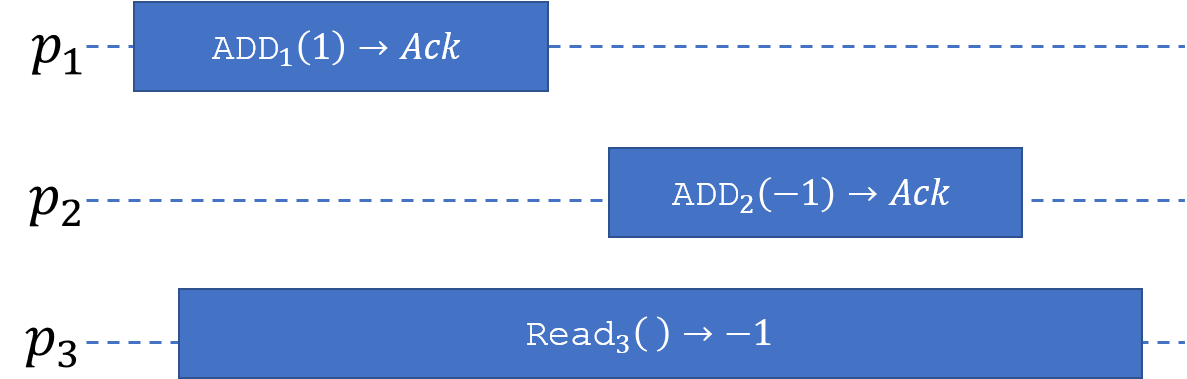
\includegraphics[width=0.5\textwidth]{images/negativeValues.png}
    \caption{A concurrent history for an adder object with four processes. $p_1$ and
    $p_2$ add $1$ and $-1$ respectively, while $p_3$ reads. $p_3$ reads $v[1]$
    before $p_1$ writes, thereby reading $0$, followed by $p_1$ and $p_2$ finishing their writes.
    Finally $p_3$ completes its read, returning $-1$.}
    \label{ivl-img:negative-values}
\end{figure}

We define a \emph{parameter} object, which supports operations {\sc update}($v$) such that $v \in \mathds{R}$ and
{\sc read}(). In a similar fashion to the adder object, the sequential specification
of the parameter object is that the read returns the sum of all the values passed to
the {\sc update} operations that precede it, and $0$ if no such operation exists.

\begin{algorithm}
    \begin{algorithmic}
        \State shared adder $a_p, a_n$ \Comment{Shared adders for positive and negative numebrs}
        \Statex
        \Procedure{update$_i$}{$v$}
        \If{$v \geq 0$}
        \State $a_p$.{\sc update}$_i$($v$)
        \Else
        \State $a_n$.{\sc update}$_i$($-1 \cdot v$)
        \EndIf
        \EndProcedure
        \Statex
        \Procedure{read}{}
        \State $v_1 \gets a_p$.{\sc read}()
        \State $v_2 \gets a_n$.{\sc read}()
        \State $v_3 \gets a_p$.{\sc read}()
        \State $v_4 \gets a_n$.{\sc read}()
        \State \textbf{return} $\max \{v_1, v_3\} - \max \{v_2, v_4\}$
        \EndProcedure
    \end{algorithmic}
    \caption{Algorithm for IVL parameter object.}
    \label{ivl-alg:ivl-parameter}
\end{algorithm}

We implement this object using two IVL adders, $a_p$ and $a_n$. When a process wishes to
update with a positive value, it does so by adding to $a_p$, otherwise, it adds the value to $a_n$.
This implementation is wait-free and built from SWMR registers only,
with a step complexity of $O(1)$ for {\sc update} operations and $O(n)$
for {\sc read} operations. Algorithm~\ref{ivl-alg:ivl-parameter} presents our implementation of an IVL parameter object.


Furthermore, we show that as both adders are IVL, this implementation is IVL:
\begin{lemma}
    Let $a_1,a_2,\dots, a_k$ be $k$ IVL adder objects. Let $a=\sum_{i=1}^k \alpha_i \cdot a_i$ be a linear
    combination of the $k$ adders. Then object $a$ is also IVL.
    \label{ivl-lmma:combination}
\end{lemma}
\begin{proof}
    Let $a_1, \dots, a_k$ and $\alpha_1, \dots, \alpha_k$ be as defined in the lemma.
    Consider some adder $j$. As it is IVL, there exist two values $v_j^1, v_j^2$ such if
    the read returns $v_j$, such that $v_j^1 \leq v_j \leq v_j^2$. Consider $\alpha_j \cdot v_j$.
    If $\alpha_j > 0$, then $\alpha_j \cdot v_j^1 \leq \alpha_j \cdot  v_j \leq \alpha_j \cdot v_j^2$,
    otherwise the inequality flips, and we get $\alpha_j \cdot v_j^2 \leq \alpha_j \cdot  v_j \leq \alpha_j \cdot v_j^1$.
    Either way, there exist $v_j^{1'}, v_j^{2'}$ such that $v_j^{1'} \leq \alpha_j \cdot  v_j \leq v_j^{2'}$.

    Consider $v = \sum_{i=1}^k \alpha_i \cdot v_i$ as read by $a$. Then:
    \begin{equation}
        \sum_{i=1}^k v_i^{1'} \leq v \leq \sum_{i=1}^k v_i^{2'}
    \end{equation}

    Furthermore, when replacing the read values with the appropriate bounds the histories of $a_1, \dots, a_k$ are linearizable.
    Therefore by composing them we get a linearizable object~\cite{herlihy1990linearizability}. Therefore the linear
    combination of IVL adder objects gives an IVL object.
\end{proof}

With Lemma~\ref{ivl-lmma:combination}, we have shown the following theorem:
\begin{theorem}
    There exists a wait-free IVL implementation of a parameter object using only SWMR registers,
    such that the step complexity of {\sc update} is $O(1)$
    and the step complexity of {\sc read} is $O(n)$.
\end{theorem}

The lower bound proved in Section~\ref{ivl-sec:lower-bound} holds here too, as the reduction can be
done using an update object instead of an adder object, and the proof remains the same. Therefore,
we get the following theorem:
\begin{theorem}
    For any linearizable wait-free implementation of an parameter object with $n$ processes from SWMR registers, the step-complexity
    of the {\sc update} operation is $\Omega(n)$.
    \label{ivl-thm:lower-bound}
\end{theorem}

%%
%% The acknowledgments section is defined using the "acks" environment
%% (and NOT an unnumbered section). This ensures the proper
%% identification of the section in the article metadata, and the
%% consistent spelling of the heading.
%\begin{acks}
%To Robert, for the bagels and explaining CMYK and color spaces.
%\end{acks}

%%
%% The next two lines define the bibliography style to be used, and
%% the bibliography file.
%\bibliographystyle{ACM-Reference-Format}
\bibliographystyle{ACM-Reference-Format}% the mandatory bibstyle`
\bibliography{bibliography}

%\newpage

%\appendix

%

\pagestyle{empty}

\section*{Appendix}

\section{Locality proof}
\label{ivl-sec:locality-proof}
We now prove that IVL is a local property:
\local
\begin{proof}
    Let $A$ be a deterministic algorithm, and let $\mathcal{H}_x$ be the sequential specification of object $x$, for every $x \in \mathcal{X}$.
    The ``only if'' part is immediate.
  
    Denote by ${H_1^x}, {H_2^x}$ the linearizations of ${H|_x}^?$ guaranteed by the
    definition of IVL.
    We first construct a linearization $H_1$ of $H^?$, defined
    by the order $\prec_{H_1}$ as follows: For every pending operation on object $x$, we either
    add the corresponding response or remove it based on ${H_1^x}$. We then construct a partial order
    of operations as the union of $\{{\prec}_{H_1^x}\}_{x \in \mathcal{X}}$ and the realtime order
    of operations in $H$. As ${\prec}_{H_1^x}$ must adhere to the realtime order of $H|_x$,
    and therefore $H$, and the order of operations in $\{{\prec}_{H_1^x}\}_{x \in \mathcal{X}}$ are disjoint, this partial order
    is well defined. Consider two concurrent operations $op_1, op_2$ in $H$. If they
    do not belong to the same history $H|_x$ for some object $x$, we order them arbitrarily in $\prec_{H_1}$.
    We construct linearization $H_2$ of $H^2$ by defining the order of operations $\prec_2$ in a similar fashion.
  
    By construction all invocations and responses appearing in $H^?$ appear both in $H_1$ and in $H_2$,
    and $H_1$ and $H_2$ preserve the partial order $\prec_{H^?}$. Therefore, $H_1$ and $H_2$ are linearizations
    of $H^?$.
    
    Consider some read $R$ on some object $x \in \mathcal{X}$ that returns in $H$. As $H|_x$ is IVL
    $\text{ret}(R,  \tau_{\mathcal{H}_x}(H_1^x) \leq \text{ret}(R, H|_x) \leq \text{ret}(R, \tau_{\mathcal{H}_x}(H_2^x))$.
    Note that $\text{ret}(R, H|_x) = \text{ret}(R, H)$. Furthermore, $\text{ret}(R, \tau_{\mathcal{H}_x}(H_i^x))= \text{ret}(R, \tau_{\mathcal{H}}(H_i))$ for $i \in \{1,2\}$,
    as objects other than $x$ do not affect the return value of this operation. Therefore $H$ is IVL.
  \end{proof}


\end{document}
\endinput
%%
%% End of file `sample-sigconf.tex'.
